% !TEX TS-program = xelatex
% !TEX encoding = UTF-8 Unicode
% !Mode:: "TeX:UTF-8"
\documentclass[bachelor,nocolorlinks, printoneside]{seuthesis} % 本科
% \documentclass[master]{seuthesis} % 硕士
% \documentclass[doctor]{seuthesis} % 博士
% \documentclass[engineering]{seuthesis} % 工程硕士
\usepackage{ctex}
\usepackage{CJK,CJKnumb}
\usepackage{amsmath}
\usepackage{amsfonts} 
\usepackage{bm} 
\usepackage{algorithm}
\usepackage{algorithmicx}
\usepackage{algpseudocode}
\usepackage{subfigure}
\usepackage{latexsym}
\usepackage{amsthm}
\usepackage{enumitem}
\usepackage{multirow}
\usepackage[section]{placeins}
\usepackage{float}
\usepackage{indentfirst} 
\usepackage{booktabs}
\usepackage{enumerate}
\usepackage{amssymb}

\floatname{algorithm}{算法}
\renewcommand{\algorithmicrequire}{\textbf{输入:}}
\renewcommand{\algorithmicensure}{\textbf{输出:}}
 % 这里是导言区

\begin{document}

\categorynumber{000} % 分类采用《中国图书资料分类法》
\UDC{000}            %《国际十进分类法UDC》的类号
\secretlevel{公开}    %学位论文密级分为"公开"、"内部"、"秘密"和"机密"四种
\studentid{04015124}   %学号要完整,前面的零不能省略。

\title{大规模MIMO的检测与估计}{}{Detection and Estimation of Massive MIMO System}{subtitle}
\author{郑奕飞}{Yifei Zheng}
\advisor{孙晨}{讲师}{Chen Sun}{Prof.}
\coadvisor{王闻今}{副教授}{Wenjin Wang}{Associate Prof.} % 没有

% \degree{工学硕士} % 详细学位名称
\major[12em]{信息工程}
\defenddate{答辩日期}
\authorizedate{学位授予日期}
\department{信息科学与工程学院}{department name}
\duration{2019年1月1日—2019年6月5日}
\address{无线谷1405室}
\maketitle

\begin{abstract}{大规模MIMO, 波束域信道模型, MMSE检测, 低复杂度检测,PE接收机}
目前流行的物联网,智能互联,车联网,天地融合等新兴技术需要大吞吐,低时延,低功耗,硬件要求低的通信系统,所以在第四代移动通信系统基础上,第五代移动通信系统(5G,5th Generation)将进一步提高这些指标。大规模MIMO技术可以显著提升系统的频谱效率和功率效率,是5G移动通信的关键技术。在大规模MIMO上行传输中,基站根据接收信号,恢复各用户的发送信号。因为天线数量多,信道复杂,一般的检测方法的复杂度将会非常高。本论文将以此为研究背景,推导适用大规模MIMO的低复杂检测算法。

首先,建立大规模MIMO传输信道模型,并研究了大规模MIMO信道特性。本文从物理多径信道模型出发,分析了物理信道模型的参数含义,并建立物理信道模型与统计信道模型的关系。进而,提出了大规模MIMO波束域信道模型,分析了大规模MIMO波束域信道的特性,包括:DFT矩阵渐近解相关、波束与方向对应性以及波束域信道稀疏性。利用3GPP空间信道模型(SCM
),生成波束域信道样本,验证波束域信道的特性,为后续章节的研究打下了基础。

然后,推导了大规模MIMO上行传输的MMSE接收机,并利用QR分解提出低复杂度接收算法。基于大规模MIMO无线传输的系统模型,阐述了上行传输中MMSE检测方法。分析MMSE检测数学表达式中复杂度最高的矩阵求逆运算,利用QR分解降低MMSE检测的计算复杂度。而利用QR分解的Givens变换在稀疏矩阵复杂度降低,以及波束域信道矩阵在经过DFT变换后信道矩阵稀疏的性质,提出了基于MMSE的低复杂度接收机。其将原始MMSE的计算复杂度$O(M^3)$($M$为基站接收天线数)化简至$O(N_uN_{beam})$($N_u$为用户数,$N_{beam}$为用户所占波束)。将基于MMSE的低复杂度接收机性能与MMSE检测结果的作对比,得出此低复杂度接收机在降低复杂度的同时很好的保持了性能的结论。

最后,利用Cayley Hamilton理论得出了相较MMSE接收机拥有更低复杂度的多项式展开(PE,Polynomial Expansion)接收机。针对MMSE检测中矩阵求逆复杂度高的问题,根据Cayley Hamilton理论,利用矩阵多项式逼近矩阵求逆结果,可以在保证一定性能的情况下将复杂度降低至$O(M^2L^2)$($L$为多项式接收机的阶数)。进而,在大规模MIMO系统中,利用算子自由概率推导了在矩阵维度较大时的确定性等同PE接收机,低复杂度的PE接收机具有本论文提出的几个低复杂度算法的最低的复杂度。利用仿真结果分析了低复杂度PE接收机的性能及复杂度$O(M^2)$。
\end{abstract}

\begin{englishabstract}{Massive MIMO, Beam Domain Channel Model, MMSE Detector, Low Complexity Detector Alogrithm, PE detector}
Nowadays, the popular new technologies such as Internet of Things, Intelligent Interconnection, Vehicle Networking, Space-Earth Integration need communication systems with high throughput, low delay, low power consumption and low hardware requirements. Therefore, the fifth generation mobile communication system (5G, 5th Generation) will further improve these indicators in the fourth generation mobile communication system. Large scale MIMO technology can significantly improve the spectrum efficiency and power efficiency of the system, and is the key technology of 5G mobile communication. In Large-Scale MIMO upstream transmission, the base station restores the transmitted signal of each user according to the received signal. Because of the large number of antennas and the complex channel, the complexity of general detection methods will be very high. In this paper, a low complexity detection algorithm for Large-Scale MIMO is deduced.

Firstly, a Large-Scale MIMO transmission channel model is established and the characteristics of Large-Scale MIMO channel are studied. Starting from the physical multipath channel model, this paper analyses the parameters of the physical channel model, and establishes the relationship between the physical channel model and the statistical channel model. Furthermore, a Large-Scale MIMO beam-domain channel model is proposed, and the characteristics of Large-Scale MIMO beam-domain channel are analyzed, including asymptotic decorrelation of DFT matrix, beam-to-direction correspondence and channel sparsity in beam-domain. Using 3GPP Space Channel Model (SCM)

To generate channel samples in the beam domain and verify the characteristics of the channel in the beam domain, which lays a foundation for the following chapters.

Then, the MMSE receiver for Large-Scale MIMO upstream transmission is deduced, and a low complexity receiving algorithm is proposed by using QR decomposition. Based on the system model of Large-Scale MIMO wireless transmission, the MMSE detection method in upstream transmission is described. The matrix inversion operation with the highest complexity in MMSE detection mathematical expression is analyzed, and the QR decomposition is used to reduce the computational complexity of MMSE detection. The Givens transform based on QR decomposition reduces the complexity of sparse matrix and the sparse property of channel matrix in beam domain after DFT transformation. A low complexity receiver based on MMSE is proposed. It simplifies the computational complexity of the original MMSE from $O(M^3) $($M $is the number of base station receiving antennas) to $O(N_uN_{beam}) $($N_u$is the number of users, $N {beam}$is the beam occupied by users). By comparing the performance of the low complexity receiver based on MMSE with the results of MMSE detection, it is concluded that the low complexity receiver can reduce the complexity while maintaining the performance well.

Finally, using Cayley Hamilton's theory, a polynomial Expansion (PE) receiver with lower complexity than MMSE receiver is obtained. For the high complexity of matrix inversion in MMSE detection, according to Cayley Hamilton theory, using matrix polynomial approximation matrix inversion results, the complexity can be reduced to $O(M^2L^2) $($L$is the order of polynomial receivers) with certain performance guaranteed. Furthermore, in Large-Scale MIMO systems, the deterministic equivalent of PE receiver is deduced by using operator freedom probability when the matrix dimension is large. The low complexity PE receiver has the lowest complexity of several low complexity algorithms proposed in this paper. The performance and complexity of the low complexity PE receiver are analyzed by simulation results, $O(M^2)$.
\end{englishabstract}

\tableofcontents


\begin{Main} % 开始正文

\chapter{绪论}
\section{研究背景}
最近30年,信息时代的技术飞速发展,移动通信技术也依托20世纪的理论基础和21世纪的硬件发展迅速,引领了21世纪的信息革命。从第一代移动通信技术(1G, 1st Generation)的模拟通信和频分多址(FDMA, Frequency Division Multiple Access)技术,到第二代移动通信技术(2G, 2nd Generation)的数字通信和时分多址(TDMA, Time Division Multiple Access)技术,到第三代移动通信技术(3G, 3th Generation)的蜂窝移动网络以及宽带码分多址(CDMA, Code Division Multiple Access)技术,到现在中国已经大面积覆盖使用的第四代移动通信技术(4G, 4th Generation)的多天线技术和正交频分复用(OFDM, Orthogonal Frequecy Division Multiple)技术。目前新兴产业如物联网,智能互联,车联网等新兴技术对大吞吐,低时延,低功耗,硬件要求低的通信系统的需求日益增高,所以第五代移动通信系统(5G, 5th Generation)将在第四代移动通信系统上进一步提高这些指标。

由于智能设备,移动设备广泛使用以及实现M2M通信的目标,全球移动通信网络所需要传输的数据量猛增。同时目前的设计受制于通信频谱的不足的问题发展到达了瓶颈。为了解决通信的数据量猛增以及低损的频谱波段的不足的问题,所以考虑使用大规模多输入多输出传输技术(LS-MIMO Large-Scale Multiple Input Multiple Output)。目前的毫米波发展导致传输相同的距离需要更高的功率或者比3G/4G更多的基站,此时也需要大规模MIMO的发展来建立适合小蜂窝的网络结构。\cite{zhang2018recent}

大规模MIMO系统影响接收信号强度主要的原因是多径传输,多普勒影响,空间特性的影响。多径的影响主要是发送端和接收端之间的有许多不同的传输路径,多普勒影响主要是移动的发送端或者接收端带来的频率偏移,大规模MIMO天线带来的波束指向性会带了空间特性。而与传统的MIMO不同的是大规模MIMO有一些特别的性质,包括更有利的发射状态,发射角特性,球形波阵面假设和空间不稳定特征。目前的大规模MIMO信道测量方式主要是利用宽带高同步率的收发机,进行大量的数据传输得到信道参数。并且针对不同情况进行不同的天线设置。目前的信道测试基本上以6GHz以下的频带进行测试,从而验证了大规模MIMO的特别性质。而未来大规模MIMO信道建模的研究方向要考虑之前提到的大规模MIMO相对于传统MIMO的特性,并且需要结合第五代移动通信采用的核心技术。

大规模MIMO检测是大规模MIMO技术的一部分,并且是基础功能。大规模MIMO检测目前主要使用的是最小均方误差估计(MMSE检测)技术,其很大的问题是MMSE检测的复杂度。因为大规模MIMO使用的天线数和用户数相较以往的普通通信系统具有更为复杂的信道,以及更大规模的信道矩阵,这对于MMSE检测来说,大规模的信道矩阵将使MMSE检测中的矩阵求逆的运算变得非常复杂。计算复杂度过大带来的问题是对于硬件的计算能力和计算时延有一定的要求,而想进一步的减少硬件和时间的开销就要求减少MMSE检测的复杂度或者是研究出接近MMSE性能的其他检测算法。时延和硬件上处理速度和所需要的资源很大程度上决定了MIMO系统的吞吐量。而提高系统的吞吐量是大规模MIMO技术的目标,所以高效,低复杂度,并行的大规模MIMO检测技术,在大规模MIMO系统中提高吞吐量起到了至关重要的作用。\cite{yang2015fifty}

选题的研究方向主要就是研究低复杂度的检测算法,并且通过建立大规模MIMO空间信道模型以及以MMSE检测作为性能评估标准验证其在降低复杂度的同时能够保持良好的性能。

\section{大规模MIMO检测与估计}
在过去五十年对于MIMO系统的检测估计做过很多研究。大规模MIMO的主要影响传输效果的原因是共通道干扰(CCI, Co-Channel Interface),而共通道干扰在MIMO中主要体现在符号间干扰(ISI, Inter Symbol Interference),通道间干扰(ICI,Inter Channel Interference),天线间干扰(IAI, Inter Antenna Interference),多用户干扰(MUI, Multiple User Interface),多接入干扰(MAI, Multiple Access Interface),多流干扰(MSI, Multiple Stream Interface)等等。而需要大规模MIMO检测的主要原因是输入信道不是相互正交,输出就会有相互干扰的情况。而应用模型主要有三种,单用户多天线MIMO的模型(Singer-user Mutiple Antanna, SM-MIMO),多用户用户单天线的MIMO模型,多用户多天线的MIMO模型。并且根据不同的通信系统情况,主要是接收部分通信技术,一般文献会考虑以下几大规模MIMO系统模型,线性无记忆MIMO系统,离散保留记忆MIMO系统,实数MIMO系统,复数MIMO系统。前面两种模型都包含有时域和频域,后面两种系统讨论的主要是系统实现的优劣。实数MIMO系统具有实数阵规模小,操作自由,复数MIMO系统具有适应多种调制方式,硬件实现简单以及在某些情况下信道容量会比实数MIMO系统要大\cite{chen2017low}。

目前用于大规模MIMO检测的算法有很多不同种,大部分都属于最小方差估计,其中包括最适MIMO检测,经典的线性MIMO检测\cite{muller2001design},基于减少干扰的MIMO检测,基于树状搜索的MIMO检测,降维MIMO检测(LR),概率数据互联MIMO检测(PDA, Probabilistic Data Association),基于半点松弛编程的MIMO检测。最适MIMO检测最先指的是ML接收机,之后几年的研究讨论了ML,MAP等估计算法的最优标准最终线性MMSE接收机确定为最优的接收机,从而也引出了关于MMSE的计算复杂度的问题。线性MIMO接收机又分为匹配滤波接收机,零干扰接收机,MMSE接收机,其他线性接收机。加性干扰去除MIMO接收机是一个非线性的接收机,效果会比线性MIMO接收机要好,而且根据不同的性质可以有很多种变种形式,性能较好的有连续干扰抵消(SIC, Successive Interference Cancellation)接收机\cite{SICD},并行干扰对消(PIC, Parallel Interference Cancellation)接收机\cite{PIC},多阶干扰对消(MIC, Multistage Interference Cancellation)接收机\cite{MICD},判决反馈接收机(DFD, Decision-Feedback Detector)\cite{DFD}\cite{DFD2}。这种接收机主要问题是如果接收信号较大,会出现错误传输的问题,更适合只需要较小信号的用户。基于树状搜索的MIMO接收机是目前研究多天线接收机的流行方向,其主要优势在于在降低接收机计算复杂度的时候可以逼近甚至达到ML接收机的效果。Lattice-Reduction(LR)接收机是基于经典的几何学和群论推导出的Lattice定义的MIMO接收机\cite{LRDetector}。其一般被用来和其他MIMO算法结合,通过优化MIMO接收机的信道矩阵优化MIMO检测算法。概率数据互联MIMO检测,PDA滤波技术是被Bar-Shalom在1975为了研究在干扰严重的环境下测量结果无法定标和结果错误时追踪和监控目标问题提出来的\cite{PDADector}。此方法本来主要是用来研究雷达追踪目标的功能来实现的。空分复用(SDM, Space-Division Multiplexing)接收机同样是为了对抗复杂环境以及降低复杂度并且取得很好的效果而提出的MIMO接收机。

大规模MIMO检测继Marzetta的开创性工作之后,LS-MIMO系统已经成为一个热门的研究课题。然而,在检测方面,一些早期的研究从大系统分析或渐进性能分析的角度探讨了这个问题。LS-MIMO系统的概念可以看作是无线通信和信号处理领域的一种范式转变。在这种大维背景下,MIMO检测问题变得更加具有挑战性和重要性。
在相关文献调查中,在线性信道上低复杂度的影响缓解可以通过使用随机矩阵理论的收敛结果可以解决优化问题。可以使用自由概率理论\cite{hachem2004simple}对MMSE检测器进行优化,使计算复杂度降低。可以利用牛顿迭代法对大规模MIMO接收机进行优化\cite{tang2016high}。同时可以利用基于坐标下降的算法对上行大规模MIMO接收机进行优化。

\section{本文工作与章节安排}
本论文以大规模MIMO系统作为所有仿真和研究的背景,主要研究的是大规模MIMO的检测技术。大规模MIMO的检测非常需要低复杂度和检测性能良好的检测方法,在大规模MIMO系统中,由于大规模MIMO的天线数巨大,所以带来检测矩阵规模也相当之大,导致常规的MIMO检测技术并不能很好的适用大规模MIMO系统。本文主要研究利用大规模MIMO性质对检测矩阵进行化简和降低复杂度的近似计算方法。论文具体安排如下:

第二章:本章叙述了大规模MIMO系统模型所需要建立的信道模型,并且研究了大规模MIMO系统信道特性。本章从物理多径信道模型出发,分析了物理信道模型的参数含义以及统计特性,并以此阐述了统计信道。进而提出了大规模MIMO的波束域信道,分析了波束域信道的特性,包括:DFT矩阵渐近解相关、波束与方向对应性以及波束域信道稀疏性。利用3GPP空间信道模型(SCM),生成波束域信道样本,验证波束域信道的特性,为后续章节的研究打下了基础。

第三章:本章叙述了检测算法的正确性所使用的系统模型,推导了大规模MIMO系统的MMSE检测,并利用QR分解提出了低复杂度MMSE算法。本章首先根据信道模型建立完整的系统模型。然后,基于大规模MIMO无线传输的系统模型,阐述了上行传输中MMSE检测方法。分析MMSE检测数学表达式中复杂度最高的矩阵求逆运算,利用QR分解降低MMSE检测的计算复杂度。而利用QR分解的Givens变换在稀疏矩阵复杂度降低,以及波束域信道矩阵在经过DFT变换后信道矩阵稀疏的性质,提出了基于MMSE的低复杂度接收机。其将原始MMSE的计算复杂度$O(M^3)$(M为基站接收天线数)化简至$O(M^2)$。将基于MMSE的低复杂度接收机性能与MMSE检测结果的作对比,得出此低复杂度接收机在降低复杂度的同时很好的保持了性能的结论。

第四章:利用Cayley Hamilton理论得出了相较MMSE接收机拥有更低复杂度的多项式展开接收机,并根据其表达式特点推导出更低复杂度检测算法。本章首先针对MMSE检测中矩阵求逆复杂度高的问题,根据Cayley Hamilton理论,利用矩阵多项式逼近矩阵求逆结果,并用仿真验证其在将复杂度降低至$O(M^2L^2)$。在大规模MIMO系统中,提出利用算子自由概率推导在矩阵维度较大时的确定性等同多项式展开接收机,低复杂度的PE接收机具有本论文提出的几个低复杂度算法的最好的复杂度。利用仿真结果分析了低复杂度多项式展开接收机的性能及复杂度$O(M^2)$。

第五章:总结了本文所做的大规模MIMO检测的工作,然后总体分析了所提出的几种算法的低复杂度和性能,通过分析提出了这几个低复杂度算法的优势与不足,并总结了未来的展望。

\section{数学符号约定}
本文在没有特殊说明的情况下,约定小写斜体表示标量,小写粗体表示向量,大写粗体表示矩阵,其他数学符号如\ref{tab:symbol}所述

\begin{table}[htbp]
	\centering
	\caption{\label{tab:symbol}数学符号约定说明}
	\begin{tabular}{ll}
		\toprule
		$(.)^H$ & 向量或矩阵的共轭转置 \\
		$(.)^T$ & 向量或矩阵的转置 \\
		$(.)^*$ & 向量或矩阵的共轭 \\
		$(.)^{-1}$ & 矩阵的逆 \\
		$\mathbb{E}[.]$ & 期望 \\
		$\odot$ & 克罗内克积 \\
		$\mathbf{I}_n$ & n维的单位矩阵  \\
		$[.]_{ij}$ & 矩阵的第i行第j列的元素 \\
		$\otimes$ & 外积 \\
		$\mathrm{diag}$ & 对角线矩阵或元素\\
		$O(.)$ & 计算复杂度 \\
		$\sqcup$ & 点集的合集 \\
		$\mathrm{Re}$ & 复数的实部 \\
		$\hat{x}$ & x的估计 \\
		$<.,.>$ & 相关\\
		$\mathrm{tr}(.)$ & 矩阵的迹 \\
		$\sum$ & 求和 \\
		$\delta$ & 冲激函数 \\
		$\mathrm{DFT}\lbrace.\rbrace$ & 离散傅里叶变换\\
		$\mathrm{IDFT}\lbrace.\rbrace$ & 离散傅里叶反变换\\
		\bottomrule
	\end{tabular}
\end{table}



\chapter{大规模MIMO信道模型}
\section{引言}
无线通信系统的性能取决于无线信道环境。无线通信信道主要描述的是无线电波从发送端传播到接收端的过程。无线通信的主要问题在于无线电波传播的过程中,无线电波会收到传播路径中物体的反射、衍射、绕射和散射。反射是指无线电波遇到相对于波长来说很大的物体表面时传播方向发生改变的物理现象,衍射是指无线电波遇到狭缝、小孔时偏离原来直线传播的物理现象,绕射是指无线电波绕过障碍物向前传播的物理现象,散射是指无线电波遇到不光滑表面时扩散传播的物理现象。为便于表述,常把对无线电波传播产生反射、衍射、绕射和散射的各类物体,统称为散射体。相应地,各非直射传播路径均称为散射路径。而对这部分传输过程以及其他原因所对信号产生的影响对其进行数学建模,具有其特征的数学模型就可以称为是无线信道。

\begin{figure}[htbp!]
	\centering 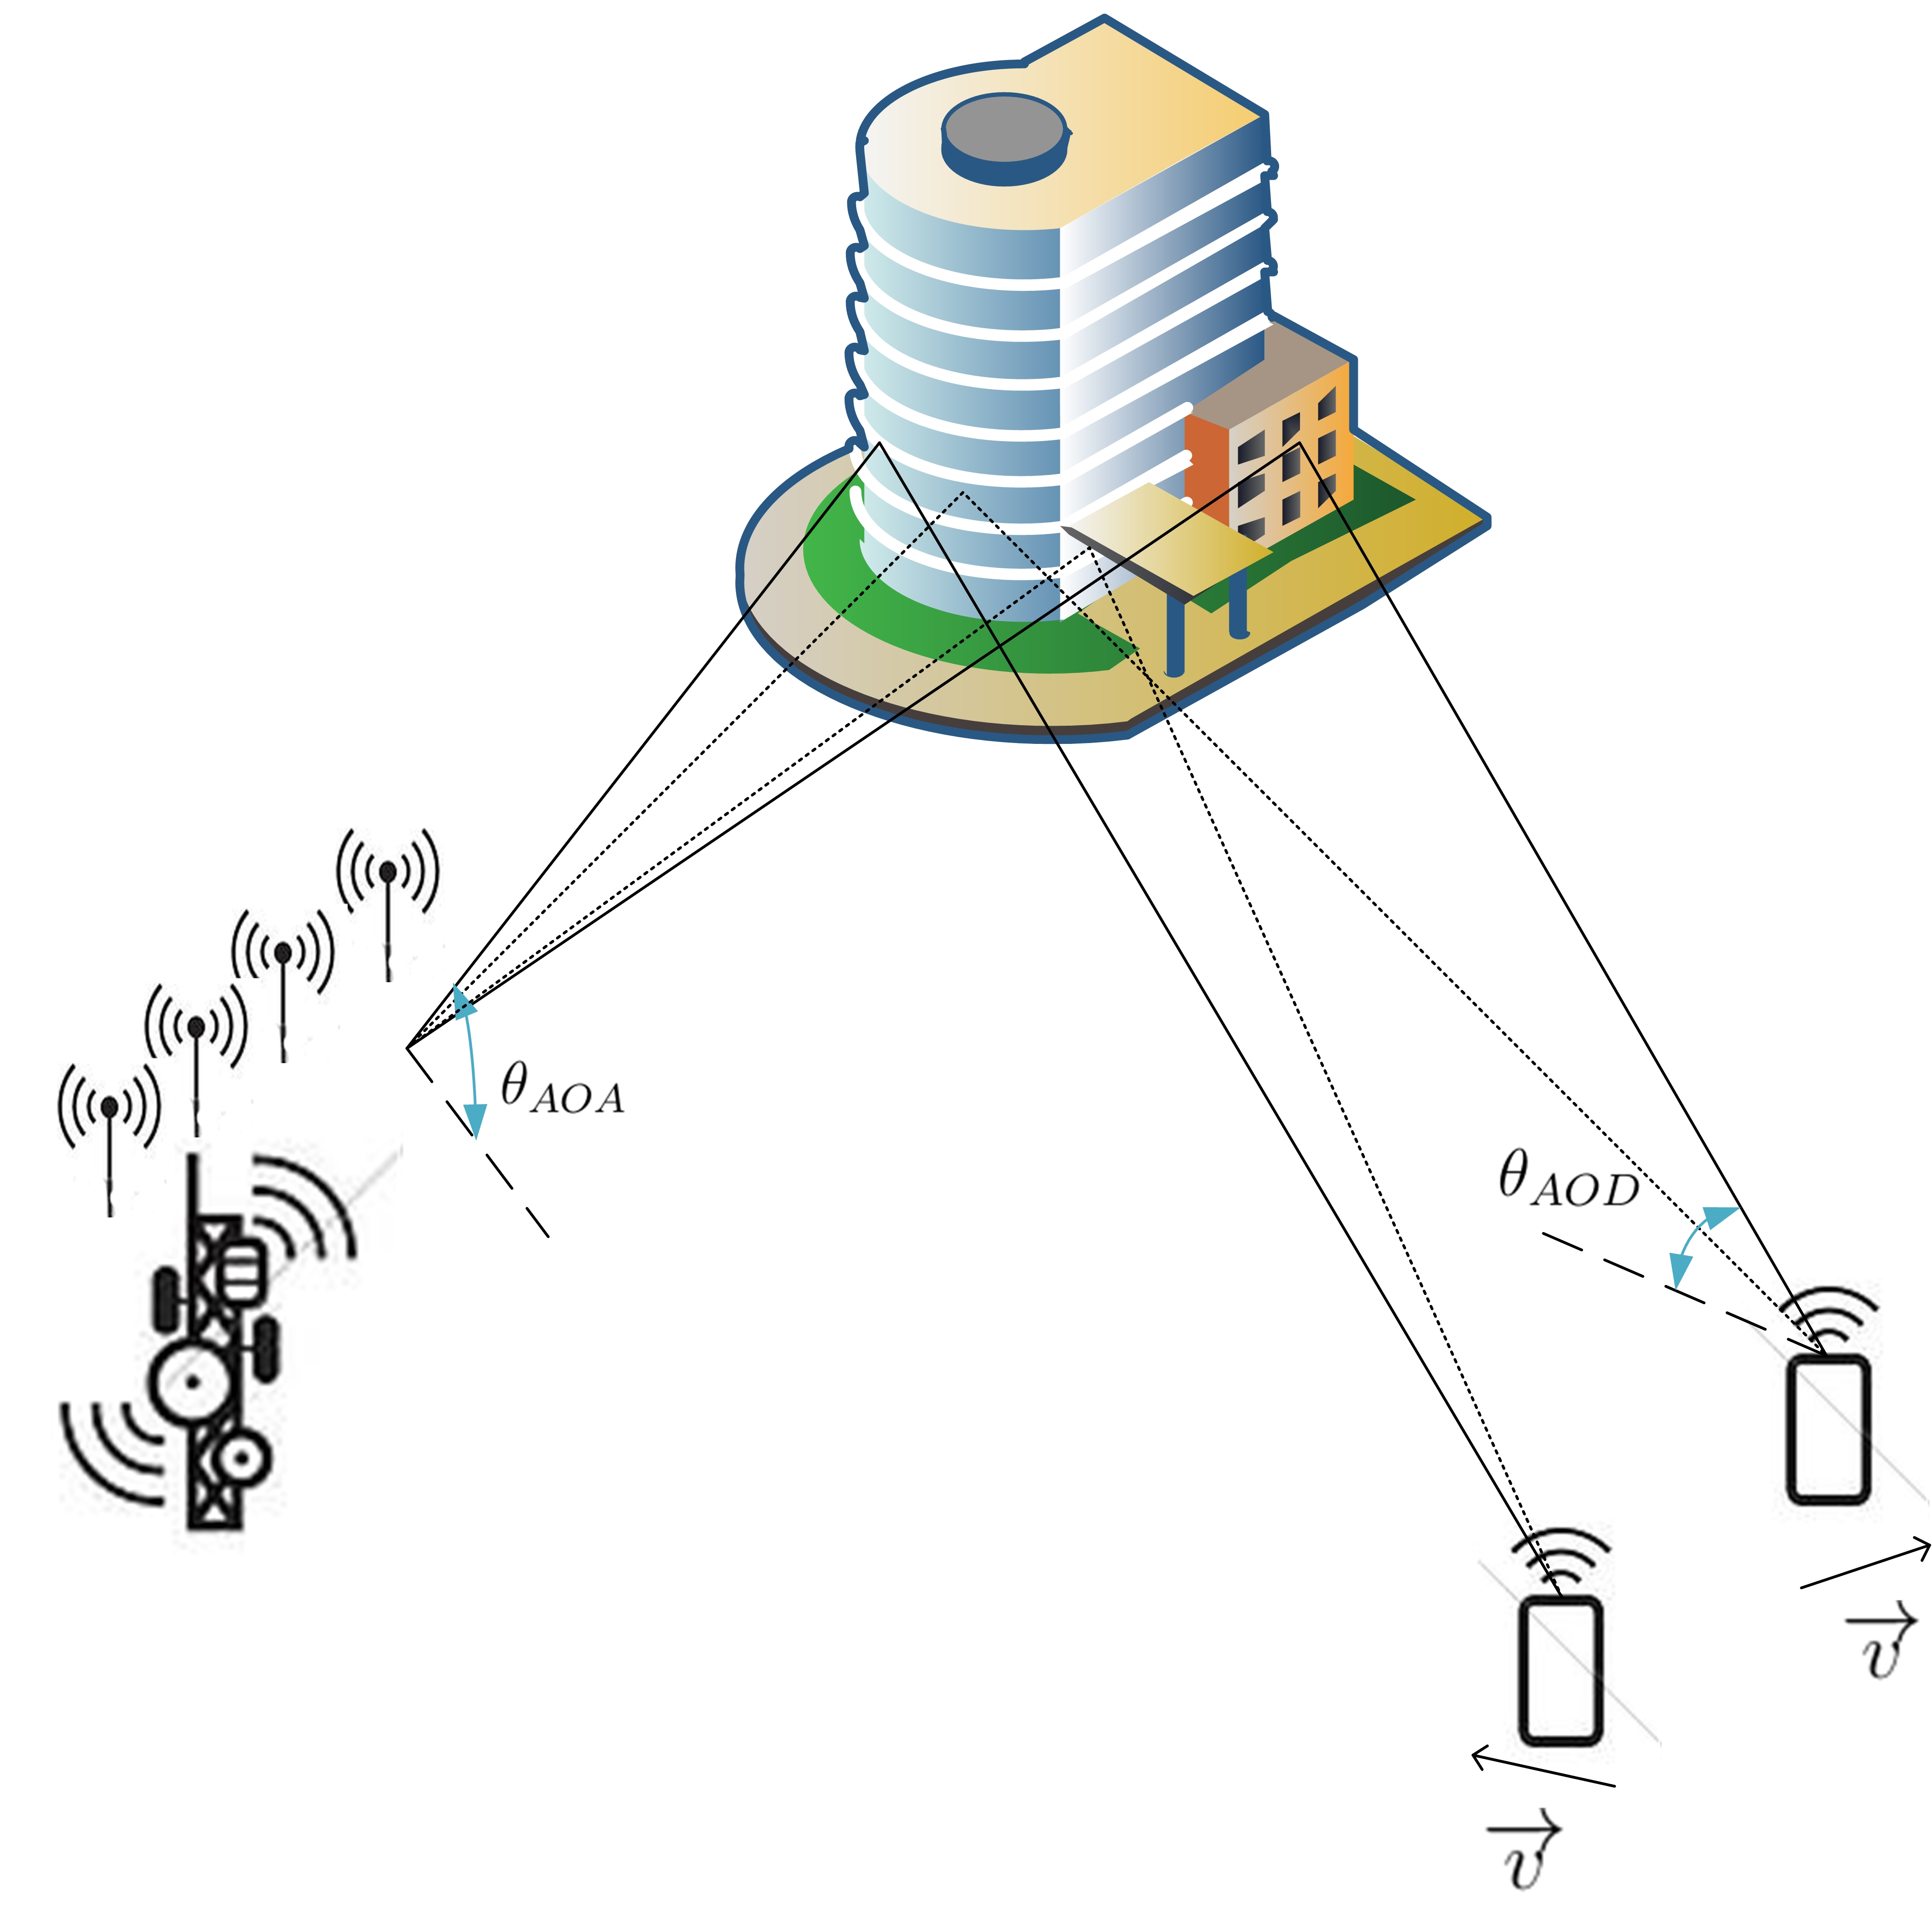
\includegraphics[width=0.45\textwidth]{img/2_1.jpg} \caption{MIMO场景示意图}
\end{figure}

无线信道的一个特有的特征是衰落,同样也是信道讨论的关键。经过无线信道传播的信号,其幅度随时间和频率变化。信号的衰落分为大尺度衰落和小尺度衰落。大尺度衰落包括与传播距离有关的路径损耗和大障碍物引起的阴影衰落,小尺度衰落是多径信号叠加和移动台移动引起的信号快速起伏变化。一般会将这两个特征分别进行数学建模,根据研究目标不同,对两种衰落的建模细致程度也会不一样。而本文讨论的大规模MIMO信道还会涉及到MIMO天线阵列对信号传输造成的影响和大规模阵列与普通MIMO信道的不同。



\section{MIMO信道物理模型}
本论文考虑的是上行信道即基站侧接收用户信息的信号检测,本文MIMO模型考虑为固定基站,配备$N_{R}$根天线,移动用户终端配备$N_{T}$根天线,其移动以$\overrightarrow{v}$表示。而城市中信道模型主要考虑的是信号传输在其中的多径情况,信号经过不同的物体表面会出现发射吸收等情况,导致最后到达接收端出现衰落,时延和相位变化。并且考虑到用户终端是移动的,会产生不同径上不同程度上的多普勒频偏。并且MIMO模型与一般的SISO模型不相同的地方在于天线阵列会提供天线阵列带来的发射和接收增益,所以本文将信道模型写为如下形式
\begin{equation}\label{key}
h_{n_{R},n_{T},p}(t) = \sum_{q=1}^{Q_{p}}u_{n_{R},p,q}h_{p,q}(t)w_{n_{T},p,q}
\end{equation}
其中,$Q_p$代表的是单个径所拥有的子径数量,$p$指的是第p径。
\begin{eqnarray}\label{key}
h_{p,q}(t) &=& \alpha_{LNA}\beta\alpha_{PA}a_{p,q}e^{j(2\pi 
	(v_{p,q}t-f_{c}\tau_{p,q}-v_{p,q}\tau_{p,q})+\phi_{p,q}
	)} \\
w_{n_{T},p,q} &=& \mathrm{exp}(-j2\pi \frac{d_{n_{T}}}{\lambda}\sin \theta_{p,q,AOD})\\
u_{n_{R},p,q} &=& \mathrm{exp}(-j2\pi \frac{d_{n_{R}}}{\lambda}\sin \theta_{p,q,AOA})
\end{eqnarray}
式(2.2)意义是信道多径带来的信道响应,式(2.3)(2.4)意义是天线阵列带来的信道响应
其中$ v_{p,q} $为多普勒频移 $ v_{p,q} = \frac{v}{\lambda}\cos\theta_{v,p,q} $ 为用户端移动带来的影响$ \phi_{p,q} $为相位变化,$\tau_{p,q}$为传播带来的时延,$d_{n_{T}}$为第$n_T$根天线与第一根天线的距离,$d_{n_{R}}$为第$n_R$根天线与第一根天线的距离,$\theta_{p,q,AOD}$表示的是第p径的第q个子径的离开角,$\theta_{p,q,AOD}$表示的是第p径的第q个子径的到达角

以下主要讨论的是信道的特征,首先是信道小尺度衰落的特征,
式(2.2)中$a_{p,q}$为相位信号幅度衰减,$\tau_{p,q}$为传播带来的时延,其中时延拓展一般分为最大时延拓展和均方根时延拓展,最大时延拓展定义为最大时延径和最小时延径的时延差,均方根时延拓展分别定义为
\begin{equation}\label{key}
\sigma_{\tau} = \sqrt{ 
	\frac{
		\sum_{p=1}^{P}(\tau_{p}-\overline{\tau})P(\tau_{p})
	}
	{
		\sum_{p=1}^{P}
		P(\tau_{p})
	}
}
\end{equation}
其中,$\tau_p$指的是各个子径的平均时延,$P(\tau_{p})$指的是子径时延所占比例,$\overline{\tau}$可以用下式定义
\begin{equation}\label{key}
\overline{\tau}=\frac
{\sum^{P}_{p=1}\tau_{p}P(\tau_{p})}
{\sum_{p=1}^{P}P(\tau_{p})}
\end{equation}
通常因为不同径距离不同而带来的通过时间的差异,所以一般时延拓展一般多会考虑时延的统计特性。

用$\beta$来表示大尺度衰落,大尺度衰落一方面指的是接收信号功率随着距离的减少,被称为路径损耗,另一方面指的是接收信号功率由于阴影造成的随机衰减,被称为随机衰落。结合两种主要大尺度衰落,一般为了方便计算可以简单的建模为,单位为分贝
\begin{equation}\label{key}
\beta=10 \log_{10} K-10 \gamma \log_{10} \frac{d}{d_{0}}-\psi_{dB}
\end{equation}
其中,$K$是一个常系数,由天线的固有性质决定。$d_{0}$为天线远场的参考距离,$d$为收发端之间的距离,$\psi_{dB}$是零均值,方差为$\sigma_{\psi_{dB}}$的高斯变量。即$10 \log_{10} K $ 为天线的增益,$ 10 \gamma \log_{10}$ 为路径距离带来的影响,研究表明随着路径的增长,路径损耗趋势成指数级,而一般认为在系统定义的远场距离之外才呈现这样的性质,在远场距离之内的一般不考虑这种建模方式,$\gamma$ 一般是考虑载波的频率和天线高度所得出的,$ \psi_{dB}$ 即为随机衰落,主要是由于阴影衰落的带来的,一般建模为log-normal模型
\begin{equation}\label{key}
p(\psi)=\frac{\xi}{\sqrt{2\pi}\sigma_{\psi_{dB}\psi}}\exp\left({-\frac{(10\log_10 \psi - \mu_\psi)^{2}}{2\sigma_{\psi_{dB}}^{2}}}\right),\quad \psi > 0
\end{equation}
而如上面所述,一般单位设置为dB,则改写为下式,并一般以其的高斯分布表示
\begin{equation}\label{key}
p(\psi)=\frac{1}{\sqrt{2\pi}\sigma_{\psi_{dB}}}\exp\left({-\frac{(\psi_{dB} - \mu_\psi)^{2}}{2\sigma_{\psi_{dB}}^{2}}}\right),\quad \psi > 0
\end{equation}
此外,有些考虑视界传输信道(LOS)会将大尺度建模为自由空间传输路损模型。

式(2.3)(2.4)代表的天线阵列信道响应,其中,$d_{n_{T}}$ 表示第$n_{T}$根发送天线与第一根发射天线的距离,$d_{n_{R}}$ 表示第$n_{R}$根接收天线与第一根接收天线的距离。$\theta_{p,q,AOD}$表示的是第p径的第q个子径的离开角,$\theta_{p,q,AOD}$表示的是第p径的第q个子径的到达角。因为基站侧天线阵列天线间隔会导致天线接收到的数据相位上的不同,导致接收天线具有一定的方向性,同理可以推导至发射端以及发射天线,在这种情况下到达角$\theta_{p,q,AOD}$和离开角$\theta_{p,q,AOD}$会比较重要。

对于式(2.2)代表的多径衰落,在不考虑阵列增益时$h_{n_{R},n_{T},p}(t)$是很多个子径之和,子径可以由服从均匀分布的复数表示,这里的$Q_{p}$是比较大,所以一般将$h_{p}(t)$考虑建模为两种信道模型。一种是不考虑直达径的瑞利衰落信道,这里讲$h_{p}(t)$建模为均值为零,方差为$\sigma_{p}^{2}$的复高斯分布随机变量。同时,因为是经过不同的散射体,各径之间相互独立,对于不同的$p_{1}$和$p_{2}$,$h_{p_{1}}$和$h_{p_{2}}$是统计独立的。另一种是考虑直达径的瑞信衰落信道,即第一个径包括直达径,$h_{1}$建模为均值非零的复高斯随机变量,幅值满足瑞信分布。在MIMO模型中因为需要考虑阵列带来的接收和发送增益,所以还需要考虑信道模型中的阵列向量响应。

P径的信道的矩阵形式如下
\begin{equation}\label{key}
\mathbf{H}_{p}(t) = \left[ \begin{array}{cccc}
h_{1,1,p}(t) & h_{1,2,p}(t) & \ldots & h_{1,N_{T},p}(t) \\
h_{2,1,p}(t) & h_{2,2,p}(t) & \ldots & h_{2,N_{T},p}(t) \\
\vdots & \vdots & \ddots & \vdots \\
h_{N_{R},1,p}(t) & h_{N_{R},2,p}(t) & \ldots & h_{N_{R},N_{T},p}(t)
\end{array} \right] 
\end{equation}
由此,信道矩阵表示为
\begin{equation}\label{key}
\mathbf{H}(t,\tau) = \sum_{p=1}^{P}\mathbf{H}_{p}(t)\delta(\tau-\tau_{p})
\end{equation}
写成矩阵形式为
\begin{equation}\label{key}
\mathbf{H}(t) = \left[ \begin{array}{cccc}
\sum_{p=1}^{P}h_{1,1,p}(t) & \sum_{p=1}^{P}h_{1,2,p}(t) & \ldots & \sum_{p=1}^{P}h_{1,N_{T},p}(t) \\
\sum_{p=1}^{P}h_{2,1,p}(t) & \sum_{p=1}^{P}h_{2,2,p}(t) & \ldots & \sum_{p=1}^{P}h_{2,N_{T},p}(t) \\
\vdots & \vdots & \ddots & \vdots \\
\sum_{p=1}^{P}h_{N_{R},1,p}(t) & \sum_{p=1}^{P}h_{N_{R},2,p}(t) & \ldots & \sum_{p=1}^{P}h_{N_{R},N_{T},p}(t)
\end{array} \right]
\end{equation}

本论文讨论的是窄带信号,但是需要注意的是,在考虑宽带情况下,信道都具有具有时间选择性和频率选择性。除此以外,MIMO信道还具有空域选择性,这一特性会导致MIMO信道矩阵各元素具有相关性。信道的功率角度谱和角度拓展用来表示MIMO信道的空域选择性,以$P(\theta_{AOA})$表示到达角为$\theta_{AOA}$方向上信道幅值的均方值,反映$\theta_{AOA}$方向上的平均接收功率,称为信道的功率角度谱。均方根角度拓展定义为
\begin{equation}\label{key}
\sigma_{\theta_{AOA}}=\sqrt{
	\frac{\int_{-\pi}^{\pi}(\theta_{AOA}-\overline{\theta}_{AOA})P(\theta_{AOA})d\theta_{AOA}}
	{\int_{-\pi}^{\pi}P(\theta_{AOA})d\theta_{AOA}}
}
\end{equation}

\section{MIMO信道统计模型}
从式(2.10)可以得到$\mathbf{H}$是一个$N_{R} \times N_{T}$矩阵。考虑该情况下的联合相关信道
\begin{equation}\label{key}
\mathbf{H} = \mathbf{U}_{r}\tilde{\mathbf{H}}\mathbf{U}_{t}^{H} = \mathbf{U}_{r}(\mathbf{D}+\mathbf{M}\odot \mathbf{H}_{idd})\mathbf{U}_{t}^{H}
\end{equation}
其中$\tilde{\mathbf{H}} = \mathbf{D}+\mathbf{M}\odot \mathbf{H}_{idd}$,$\mathbf{U}_{t}$和$\mathbf{U}_{r}$分别是$N_{T} \times N_{T}$维 和$N_{R} \times N_{R}$维的确定酉矩阵。$\mathbf{D}$是一个$N_{R} \times N_{T}$维每行每列至少有一个非零元素的确定性矩阵,$\mathbf{M}$是一个$N_{R} \times N_{T}$维非负确定矩阵,$\mathbf{H}_{i.i.d.}$是一个$N_{R} \times N_{T}$维零均值独立同分布的矩阵。$\mathbf{H}_{i.i.d.}$并不限于是高斯。但本文在上述条件下考虑的是单位方差的高斯矩阵。由上式(2.15)一般定义
\begin{equation}\label{key}
\bm{\Omega} =\mathbb{E}[\tilde{\mathbf{H}} \odot \tilde{\mathbf{H}}^{*}]
\end{equation}
即
\begin{equation}\label{key}
\bm{\Omega} = \mathbf{D} \odot \mathbf{D} + \mathbf{M} \odot \mathbf{M}
\end{equation}
则有
\begin{eqnarray}\label{key}
\mathbf{D} & = & \mathbb{E}[\tilde{\mathbf{H}}] \\
\left[  \mathbf{M} \right]_{ij} & = & \sqrt{\mathrm{var}(\tilde{[\mathbf{H}]}_{ij})} \nonumber \\
& = & \sqrt{[\bm{\Omega}]_{ij}-[D]_{ij}^{2}}
\end{eqnarray}
即矩阵$\mathbf{D}$和$\mathbf{M}$分别代表了信道的LOS和信道的稀疏元素所以又称$\bm{\Omega} $为特征能量耦合矩阵,可以看出特征能量耦合矩阵$\bm{\Omega}$的各行各列是信号传输过程中发送端和接收端相关矩阵的集合,这些本征值是不可分解的,并且代表了信道的联合相关特征。并且根据上述性质,其可以改写发射功率约束为
\begin{equation}\label{key}
\sum_{i=1}^{N_{R}}\sum_{j=1}^{N_{T}}[\bm{\Omega}]_{ij} = N_{T}N_{R}
\end{equation}
又因为式(2.14),可以将发射和接收端的协方差矩阵写为
\begin{eqnarray}\label{key}
\mathbf{R}_{t}=\mathbb{E}\lbrace \mathbf{H}^{H}\mathbf{H} \rbrace = \mathbf{U}_{t}\bm{\Lambda}_{t}\mathbf{U}_{t}^{H} \\
\mathbf{R}_{r}=\mathbb{E}\lbrace \mathbf{H}\mathbf{H}^{H} \rbrace = \mathbf{U}_{r}\bm{\Lambda}_{t}\mathbf{U}_{r}^{H}
\end{eqnarray}
$\bm{\Lambda}_{t}$和$\bm{\Lambda_{r}}$是对角阵,并有
\begin{eqnarray}\label{key}
[\bm{\Lambda}_{t}]_{ii} & = & \sum_{j=1}^{N_{r}} [\bm{\Omega}]_{ji} 
\end{eqnarray}
由此可以说明$\mathbf{U}_{t}$和$\mathbf{U}_{r}$是发送端和接收端协方差矩阵的特征向量矩阵。这些矩阵元素由天线的特性决定。本论文主要讨论的天线阵列为均匀线阵(ULA),所以特征向量矩阵也可以直接写为离散傅里叶变换矩阵(DFT)。

上面推导的联合概率模型是一个泛式,根据$ \mathbf{D}$和$\mathbf{M}$不同取值,可以分为不同的联合概率模型。例如,当$\mathbf{D}=0,\mathbf{M}$是一个秩为1的矩阵,$\mathbf{H}_{i.i.d.}$有瑞利衰落信道,则上述模型为分离相关Kronecker模型。当令$\mathbf{M}$的秩为随机值,将$\mathbf{U}_t$和$\mathbf{U}_t$固定为DFT矩阵,此时获得的信道模型为均匀线阵天线系统的虚拟信道模型。在这基础上,令$\mathbf{U}_t$和$\mathbf{U}_r$为随机酉矩阵,得到的为Weichselberger模型。本论文考虑的主要是在Weichselberger模型基础上令$ \mathbf{D} = 0 $的UIU模型。

除此之外,还有一种常用MIMO信道统计模型是分离相关信道模型,也称为直积信道模型,一般表示为$ \mathbf{H} = \bm{\Theta}_R^{1/2} \mathbf{H}_{i.i.d.} \bm{\Theta}_T^{1/2}$其一般不考虑信道时变特性,并且联合相关信道模型更加贴近实际,所以本论文不考虑直积信道模型的作用。

\section{大规模MIMO波束域信道模型}
推导波束域信道模型,需要预先分析大规模MIMO的空间信道特征\cite{SunchenBD}\cite{Youli2},考虑上文提到的物理信道模型式(2.1)和式(2.2),为了后续化简可以将其改写为矩阵形式并合并一些本论文不作具体建模的变量
\begin{equation}\label{key}
\mathbf{H} = \sum_{p=1}^{P}\beta_p \mathbf{u}_{r,p}\mathbf{w}_{t,p}e^{-j2\pi \tau_{p,k}}
\end{equation}
$\beta_p$表示第p径带来的总体增益其中包括之前提到的发射接收增益以及路径衰落。本论文考虑的是均匀线阵天线阵列,并且天线间隔为半波长,根据式(2.3)和式(2.4)可以将阵列响应写成如下的向量形式
\begin{eqnarray}\label{key}
\mathbf{u}_{r,p}(\theta_{AOA}) = [1,e^{-j\pi \sin \theta_{AOA}},...,e^{-j\pi (N_R-1)}\theta_{AOA}] \\
\mathbf{w}_{t,p}(\theta_{AOD}) = [1,e^{-j\pi \sin \theta_{AOD}},...,e^{-j\pi (N_T-1)}\theta_{AOD}]
\end{eqnarray}

为了将模型变换到波束域,这里需要证明一个定理,在大规模MIMO系统条件下,当基站侧天线数趋于无穷时,有离散傅里叶变换(DFT)可以作为信道的特征矩阵。在天线数趋于无穷时,不同到达角AOA的阵列响应相互独立性质,即到达角的响应集中在一个位置。
\begin{equation}\label{key}
\lim_{N_R \rightarrow \infty}\frac{1}{N_R}<\mathbf{u}(\theta_1),\mathbf{u}(\theta_2)> = \delta(\theta_1 -\theta_2)
\end{equation}

将式(2.10)的信道矩阵重写成向量的集合
\begin{equation}\label{key}
\mathbf{H} = [\mathbf{h}_1,\mathbf{h}_2,...,\mathbf{h}_{N_T}]
\end{equation}
其中,
\begin{equation}\label{key}
\mathbf{h}_m = \sum_{p=1}^{P}\beta_p e^{j\pi (n_r-1) \sin(\theta_{AOA})} \mathbf{w}_{t,p}(\theta_{AOD}) e^{-j2\pi\tau_{p}}
\end{equation}
其左乘DFT矩阵,得到信道DFT之后的矩阵
\begin{equation}\label{key}
\mathbf{H}_{F} = \mathbf{F} \mathbf{H} =[\mathbf{h}_{F,1},\mathbf{h}_{F,1},...,\mathbf{h}_{F,N_T}]
\end{equation}
$\mathbf{F}$为$N_R \times N_R $DFT矩阵,其$(n_r,n_r^{'})$元素为
\begin{equation}\label{key}
[ \mathbf{F} ]_{n_r,n_r^{'}} = \frac{1}{\sqrt{N_R}} e^{-j \frac{2\pi (n_r-1)(n_r^{*}-1)}{\mathbf{N_R}}}
\end{equation}
带入式(2.29)可得
\begin{equation}\label{key}
\mathbf{h}_{F,m} = \sum_{p=1}^{P} \beta_p \left( \sum_{i=0}^{N_R-1} \frac{1}{\sqrt{N_R}} e^{j2\pi i(0.5\sin \theta_{AOA} - \frac{N_R}{n_r-1})} \right) \mathbf{w}_{t,p}(\theta_{AOD}) e^{-j2\pi\tau_{p}}
\end{equation}
根据之前提到的性质式(2.27),当基站侧天线趋于无穷时,式(2.32)可以写成
\begin{eqnarray}\label{key}
\lim_{N_R \rightarrow \infty} \sum_{i=0}^{N_R-1} \frac{1}{\sqrt{N_R}} e^{j2\pi i(0.5 \sin \theta_{AOA} -\frac{n_r-1}{N_R})} = \left \lbrace
\begin{array}{l}
0 \quad 0.5\sin \theta_{AOA} - \frac{n_r-1}{N_R} \notin \mathbb{Z} \\
\lim_{N_R \rightarrow \infty} \sqrt{N_R}  \quad 0.5\sin \theta_{AOA} - \frac{n_r-1}{N_R} \in \mathbb{Z} 
\end{array}
\right.
\end{eqnarray}
一般考虑$ 0.5\sin \theta_{AOA} - \frac{n_r-1}{N_R} \in \mathbb{Z}$ 中$0.5\sin \theta_{AOA} - \frac{n_r-1}{N_R} $的结果只有可能是-1和0,并且AOA角和天线序号一一对应。为了简化,考虑使用如下等式,使得其的结果只可能为0,从而方便接下来的推导
\begin{eqnarray}\label{key}
\tilde{n_r} = \left \lbrace
\begin{array}{l}
n_r \quad \frac{n_r-1}{N_R} < \frac{1}{2}\\
n_r - N_R \quad \frac{n_r-1}{N_R} \geq \frac{1}{2}
\end{array}
\right.
\end{eqnarray}
从而改写上式(2.32)为
\begin{equation}\label{key}
\mathbf{h}_{F,m} = \sum_{p=1}^{P} \beta_p \left( \delta( 0.5\sin \theta_{AOA} - \frac{\tilde{n_r}-1}{N_R} ) \right) \mathbf{w}_{t,p}(\theta_{AOD}) e^{-j2\pi\tau_{p}}
\end{equation}
然后本文上面推导的统计相关信道时,得到了接收端相关阵,因为本文考虑的是上行信道,所以基站侧相关阵参考(2.22)
\begin{equation}\label{key}
\mathbf{R}_{F,r} = \mathbb{E} \lbrace \mathbf{H}_{F} (\mathbf{H}_{F})^{H} \rbrace
\end{equation}
则有相关阵的第$(i,j)$个元素为
\begin{eqnarray}\label{key}
[ \mathbf{R}_{F,r} ]_{i,j} & = &\mathbb{E} \lbrace \mathbf{h}_{F} (\mathbf{h}_{F})^{H} \rbrace  \nonumber \\
& = & \sum_{p=1}^{P} \sigma_{\beta_p}^{2} \mathbf{w}_{t}(\theta_{AOD}) \mathbf{w}_{t}^{H}(\theta_{AOD}) N_R \delta \left( 0.5\sin \theta_{AOA} - \frac{\tilde{i}-1}{N_R} , 0.5\sin \theta_{AOA} - \frac{\tilde{j}-1}{N_R} \right) \nonumber \\
\end{eqnarray}
由式(2.37)可知,当$ i \neq j$时, $ [ \mathbf{R}_{F,r} ]_{i,j} = 0$,即基站侧相关阵的为对角阵。因而当天线数趋于无穷时,DFT矩阵$\mathbf{F}$为基站侧相关阵的特征矩阵$ \mathbf{U}_{r} = \mathbf{F}$。

本文在建立统计信道模型的时候讨论了用以表示发射功率约束的特征能量耦合矩阵,上面各式推导的即为式(2.15)中的$\mathbf{U}_r$,所以用DFT矩阵可以写出特征模式能量耦合矩阵为
\begin{eqnarray}\label{key}
\bm{\Omega} & = &\mathbb{E}[\tilde{\mathbf{H}} \odot \tilde{\mathbf{H}}^{*}] \nonumber \\
& = & \sum_{p=1}^{P} \sigma_{\beta_p}^{2} [\mathbf{F} \mathbf{u}_r(\theta_{AOA}) \mathbf{w}_t (\theta_{AOD})] \odot [\mathbf{F} \mathbf{u}_r(\theta_{AOA}) \mathbf{w}_t (\theta_{AOD})]^{*}
\end{eqnarray}
如果考虑OFDM系统,上式经过变式后同样可以说明特征模式能量耦合矩阵与载波无关,即不同载波的能量分布是均匀的。

由上面推导过程,可以给出以下定义,来表示基站侧配置大规模天线阵列,上行波束域信道模型
\begin{equation}\label{key}
\tilde{\mathbf{H}} = \mathbf{F}  \mathbf{H}
\end{equation}

由于上行链路和下行链路的统计信道信息在频分双工(FDD, Frequency Division Duplexing)和时分双工(TDD, Time Division Duplexing)具有互易性,并且在前面同样提到了CSI信息可以通过反馈通道或者是双向通信传输,所以下行链路的波束域模型可以由下式定义
\begin{equation}\label{key}
\tilde{\mathbf{H}} =   \mathbf{H}\mathbf{F}^{H}
\end{equation}
通过上面的推导,易得波束域信道的两个重要空间特征:波束域信道在基站侧是不相关的;上行波束域信道描述的是基站侧对于不同到达角的特征,信道矩阵的不同列代表了不同的到达角,每一个到达角又称为一个波束,故称为波束域信道模型。

本论文考虑的是上行链路和窄带信号,所以不涉及OFDM系统和下行链路。但是从推导中容易得到信道统计信息与载波无关,并且有下式来简化模型
\begin{equation}\label{key}
\bm{\Omega}_u^T = \bm{\Omega}_d =\bm{\Omega}
\end{equation}

波束域信道模型主要是突出离散傅里叶变换矩阵(DFT)表现的天线阵列的性质,并且这种天线阵列带来的角分辨率随着天线阵列规模的增大而增大。实际系统中,天线规模是有限的,但是均匀线阵的天线阵列在数目较大的情况下,波束域信道还是很好地近似了实际信道。本文考虑的大规模MIMO信道检测与估计难度在于大规模天线矩阵带来的信道矩阵协方差矩阵维度将会非常大,普通MMSE检测复杂度在$\mathcal{O}(N_R^3)$,这是非常大的计算量。波束域信道模型需要检测估计的是信道协方差矩阵特征矩阵或者说是波束域信道矩阵,大大减少了估计参数。

此外,基站侧的信道协方差矩阵也可以写作如下简单的表示
\begin{equation}\label{key}
\mathbf{R}_r \rightarrow \mathbf{U}_r \hat{\mathbf{R}}_r \mathbf{U}^{r}
\end{equation}

依据上面的推导内容,本文还可以引出如下性质
\begin{equation}\label{key}
vec(\mathbf{H}_{k,l}) = \sum_{n=1}^{N} \sum_{m=1}^{M} [\tilde{\mathbf{H}}_{p,k}]_{nm} e^{*}_{t}(\varphi_{m} )\bigotimes e_{r}(\theta_{n,k})
\end{equation}
并计算全相关矩阵的表达形式
\begin{equation}\label{key}
\mathbf{R}_{\mathbf{H},k} = \sum_{n=1}^{N} \sum_{m=1}^{M} \mathbb{E} \lbrace [\tilde{\mathbf{H}}_{p,k}]_{nm} [\tilde{\mathbf{H}}_{p,k}]_{nm}^{H}   \rbrace \times
(e^{*}_{t}(\varphi_{m} )\bigotimes e_{r}(\theta_{n,k})) (e^{*}_{t}(\varphi_{m} )\bigotimes e_{r}(\theta_{n,k}))^{H}
\end{equation}
由上面推导,以及文献中表述,可以很清楚的发现全相关矩阵和联合相关矩阵是一致的。同时可以验证本文基站侧信道特征模式能量耦合矩阵的正确性。

本论文讨论的主要是基于波束域信道模型的低复杂度检测算法,还有一种方式是依据如下关于并行分解的方式。即一个MIMO系统可以将MIMO信道可以被看做是一系列(总数为R)的平行独立信道来解释。得益于在相互独立的信道上复用相互独立的数据,本文可以获得比单天线高R倍的数据率。

考虑一个$ M_{r}* M_{t}$MIMO信道,信道矩阵为$\mathbf{H}$并且接收端和发送端都获得了信道矩阵信息。令 $ R_{\mathbf{H}}$代表$\mathbf{H}$的秩。通过SVD,可以得到$\mathbf{H}$
\begin{equation}\label{key}
\mathbf{H}=\mathbf{U}\Sigma\mathbf{V}^{H}
\end{equation}
其中,$\mathbf{U} $和$\mathbf{V} $都是酉矩阵,$\mathbf{H}$为随机矩阵。该模型更贴近实际MIMO信道。因为$ R_{\mathbf{H}}$代表$\mathbf{H}$的秩,所以$ R_{\mathbf{H}} \leq \min(M_{t},M_{r})$。当
$\mathbf{H}$满秩,称为全散射环境。其他环境都会导致非满秩,$\mathbf{H}$元素的高相关性秩为1。通道并行分解是通过发送预编码和接收机整形得到的。
\begin{eqnarray}\label{key}
\mathbf{x} &=& \mathbf{V}\tilde{\mathbf{x}}  \nonumber\\
\tilde{\mathbf{y}}&=& \mathbf{U}^{H}\mathbf{y}  \nonumber
\end{eqnarray}
\begin{eqnarray}\label{key}
\tilde{\mathbf{y}} & = &\mathbf{U}^{H}(\mathbf{H}\mathbf{x}+\mathbf{n}) {} \nonumber\\
& = & \mathbf{U}^{H}(\mathbf{U}\Sigma\mathbf{V}^{H}\mathbf{V}\tilde{x}+\mathbf{n}) \nonumber \\
& = & \Sigma\tilde{\mathbf{x}} + \tilde{\mathbf{n}}
\end{eqnarray}
其中$\tilde{\mathbf{n}}=\mathbf{U}^{H}\mathbf{n}$。其中$\Sigma$是矩阵$ \mathbf{H}$第i条对角线的单值组成的矩阵,其余为零的矩阵。虽然该单值都与矩阵$ \mathbf{H}$相关,但是本文认为不同信道并不相干,所以认为不同信道都是独立的。由此转化为SISO模型进行处理,本文不再讨论其作用。



\section{波束域信道特性}
由上面的推导,可以得出很多波束域信道的空间特征和数学特性,下文将展开叙述波束域信道的各方面特性。本文主要讨论的波束域信道三个特性:基站侧相关阵的特征矩阵为信道的DFT矩阵;在上行系统中,信道矩阵的不同列代表了不同的到达角,每一个到达角又称为一个波束;特征矩阵具有稀疏特性。\cite{SunboAngle}\cite{Youli1}\cite{Youli2}

\subsection{DFT矩阵解相关}
在讨论基站侧相关阵的特征矩阵为信道的DFT矩阵前,本文简要介绍DFT及其性质。令$x[n],0 \leq n \leq N-1$ 代表一个离散的时间序列,$x[n]$的N点的DFT定义为
\begin{equation}\label{key}
\mathrm{DFT} \lbrace x[n] \rbrace = X[i] \triangleq \frac{1}{\sqrt{N}} \sum_{n=0}^{N-1}x[n]e^{-j2\pi ni/N},\quad 0 \leq n \leq N-1
\end{equation}
DFT等同于连续时间傅里叶变换的离散表达,所以$X[i]$代表的是时域信号$x(t)$采样信号$x[n]$的频域内容。连续时间傅立叶变换和离散傅立叶变换都是基于复指数是任何线性系统的特征函数。当然采样序列$x[n]$也可以通过反DFT从频域内容中恢复出时域信息。
\begin{equation}\label{key}
\mathrm{IDFT} \lbrace X[i] \rbrace = x[n] \triangleq \frac{1}{\sqrt{N}} \sum_{i=0}^{N-1}X[i]e^{j2\pi ni/N},\quad 0 \leq i \leq N-1
\end{equation}
利用快速傅里叶变换以及快速傅里叶反变换在硬件上可以很容易得得到DFT和反DFT的结果。

由波束域信道推导过程,基站侧相关阵的特征矩阵为DFT矩阵,DFT矩阵易得,所以可以通过DFT矩阵,参考式(2.38)可以利用DFT矩阵得出信道的相关阵,表达形式即式(2.39)
\begin{eqnarray}\label{key}
[ \mathbf{R}_{F,r} ]_{i,j} & = &\mathbb{E} \lbrace \mathbf{h}_{F} (\mathbf{h}_{F})^{H} \rbrace  \nonumber \\
& = & \sum_{p=1}^{P} \sigma_{\beta_p}^{2} \mathbf{w}_{t}(\theta_{AOD}) \mathbf{w}_{t}^{H}(\theta_{AOD}) N_R \delta \left( 0.5\sin \theta_{AOA} - \frac{\tilde{i}-1}{N_R} , 0.5\sin \theta_{AOA} - \frac{\tilde{j}-1}{N_R} \right) \nonumber
\end{eqnarray}

而波束域DFT解相关有接收矩阵与用户无关,即任意天线的接收矩阵,任意用户都可以利用同一个DFT矩阵变换到波束域,利用波束域的性质。

\subsection{对应波束}
根据上面提到的信道矩阵左乘DFT矩阵,得到信道DFT之后的矩阵
\begin{equation}\label{key}
\mathbf{H}_{F} = \mathbf{F} \mathbf{H} =[\mathbf{h}_{F,1},\mathbf{h}_{F,1},...,\mathbf{h}_{F,N_T}]
\end{equation}
$\mathbf{F}$为$N_R \times N_R $DFT矩阵,其$(n_r,n_r^{'})$元素为
\begin{equation}\label{key}
[ \mathbf{F} ]_{n_r,n_r^{'}} = \frac{1}{\sqrt{N_R}} e^{-j \frac{2\pi (n_r-1)(n_r^{*}-1)}{\mathbf{N_R}}}
\end{equation}
带入式(2.29)可得
\begin{equation}\label{key}
\mathbf{h}_{F,m} = \sum_{p=1}^{P} \beta_p \left( \sum_{i=0}^{N_R-1} \frac{1}{\sqrt{N_R}} e^{j2\pi i(0.5\sin \theta_{AOA} - \frac{N_R}{n_r-1})} \right) \mathbf{w}_{t,p}(\theta_{AOD}) e^{-j2\pi\tau_{p}}
\end{equation}
根据之前提到的性质式(2.27),当基站侧天线趋于无穷时,式(2.55)可以写成
\begin{eqnarray}\label{key}
\lim_{N_R \rightarrow \infty} \sum_{i=0}^{N_R-1} \frac{1}{\sqrt{N_R}} e^{j2\pi i(0.5 \sin \theta_{AOA} -\frac{n_r-1}{N_R})} = \left \lbrace
\begin{array}{l}
0 \quad 0.5\sin \theta_{AOA} - \frac{n_r-1}{N_R} \notin \mathbb{Z} \\
\lim_{N_R \rightarrow \infty} \sqrt{N_R}  \quad 0.5\sin \theta_{AOA} - \frac{n_r-1}{N_R} \in \mathbb{Z} 
\end{array}
\right.
\end{eqnarray}
一般考虑$ 0.5\sin \theta_{AOA} - \frac{n_r-1}{N_R} \in \mathbb{Z}$ 中$0.5\sin \theta_{AOA} - \frac{n_r-1}{N_R} $的结果只有可能是-1和0,并且AOA角和天线序号一一对应。为了简化,考虑使用如下等式,使得其的结果只可能为0,从而方便接下来的推导
\begin{eqnarray}\label{key}
\tilde{n_r} = \left \lbrace
\begin{array}{l}
n_r \quad \frac{n_r-1}{N_R} < \frac{1}{2}\\
n_r - N_R \quad \frac{n_r-1}{N_R} \geq \frac{1}{2}
\end{array}
\right.
\end{eqnarray}
通过上面推导和公式,可以发现在AOA角和天线序号一一对应,换句话说,即AOA角所对应的在波束域信道中被定义为波束。
以下将用信道模型示意图来展示大规模MIMO的波束域信道的波束特性。在此之前,本文简要介绍下所使用的信道模型。
此信道模型为3GPP空间信道模型,以多输入多输出(MIMO)无线链路参数、模型配置参数和天线参数作为输入,并输出MIMO信道矩阵。利用此信道模型,可以验证波束域信道特性以及进行检测估计的仿真环境。
考虑远场散射环境,选取仿真环境为郊区宏蜂窝模型。首先考虑单天线的情况,仿真均没有考虑大尺度衰落即路损和阴影衰落。此时均考虑的是单用户或者多用户其中一个的情况。
\begin{table}[htbp]
	\centering
	\caption{\label{tab:test}SCM仿真参数设置}
	\begin{tabular}{ll}
		\toprule
		参数 &  设置值 \\
				\bottomrule
		场景 &  郊区宏蜂窝 \\
				\bottomrule
		基站侧天线数 & 128 \\
				\bottomrule
		用户数天线	& 1 \\
				\bottomrule
		天线间距 & 0.5$\lambda$ \\
				\bottomrule
		路径数 & 6 \\
		\bottomrule
	\end{tabular}
\end{table}
	
\begin{figure}[htbp!]
	\centering 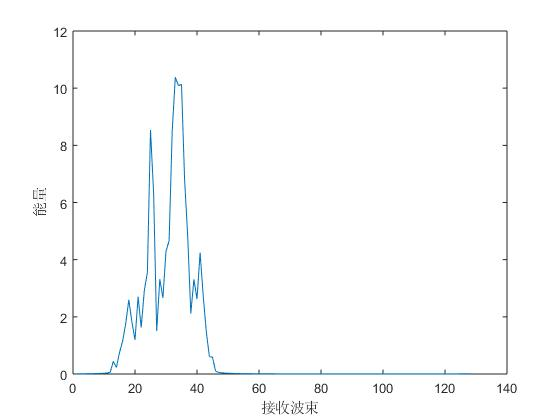
\includegraphics[width=0.6\textwidth]{img/2_2.jpg} \caption{用户单天线波束域信道能量耦合矩阵}
\end{figure}
多用户时,还可以发现,单个用户只占用部分波束,在一定情况下,可以将用户分配不同的波束,从而减少传输中不同用户的干扰,从而提高判断各用户的信号的准确度。
\begin{figure}[htbp!]
	\centering 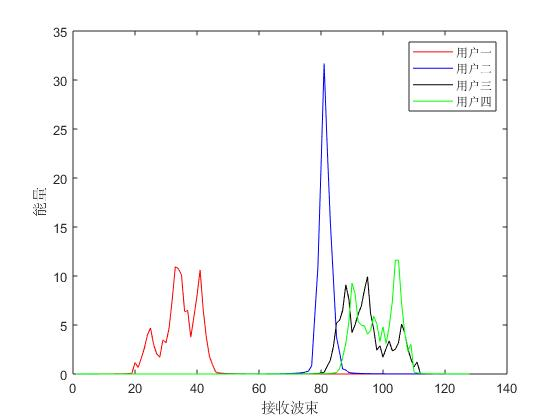
\includegraphics[width=0.6\textwidth]{img/2_5.jpg} \caption{多用户波束域信道能量耦合矩阵}
\end{figure}
考虑用户多天线的情况,此时耦合矩阵不再是单维的,所以多天线的耦合矩阵是3维视图
\begin{table}[htbp]
	\centering
	\caption{\label{tab:test}SCM仿真参数设置}
	\begin{tabular}{ll}
		\toprule
		参数 &  设置值 \\
		\bottomrule
		场景 &  郊区宏蜂窝 \\
		\bottomrule
		基站侧天线数 & 128 \\
		\bottomrule
		用户数天线	& 4 \\
		\bottomrule
		天线间距 & 0.5$\lambda$ \\
		\bottomrule
		路径数 & 6 \\
		\bottomrule
	\end{tabular}
\end{table}

\begin{figure}[htbp!]
	\centering 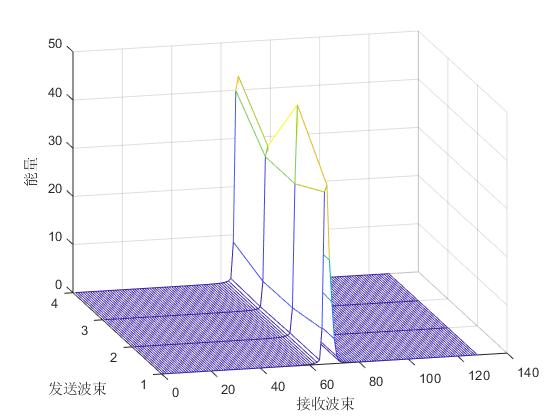
\includegraphics[width=0.6\textwidth]{img/2_3.jpg} \caption{用户多天线波束域信道能量耦合矩阵}
\end{figure}

由上面两图可以看出能量集中波束上,并且天线和AOA角对应同时也和波束对应。

\subsection{特征矩阵稀疏性}
本文上面也推导过相关阵的各元素表达式,上行信道,所以基站侧相关阵参考(2.22)
\begin{equation}\label{key}
\mathbf{R}_{F,r} = \mathbb{E} \lbrace \mathbf{H}_{F} (\mathbf{H}_{F})^{H} \rbrace
\end{equation}
则有相关阵的第(i,j)个元素为
\begin{eqnarray}\label{key}
[ \mathbf{R}_{F,r} ]_{i,j} & = &\mathbb{E} \lbrace \mathbf{h}_{F} (\mathbf{h}_{F})^{H} \rbrace  \nonumber \\
& = & \sum_{p=1}^{P} \sigma_{\beta_p}^{2} \mathbf{w}_{t}(\theta_{AOD}) \mathbf{w}_{t}^{H}(\theta_{AOD}) N_R \delta \left( 0.5\sin \theta_{AOA} - \frac{\tilde{i}-1}{N_R} , 0.5\sin \theta_{AOA} - \frac{\tilde{j}-1}{N_R} \right) \nonumber \\
\end{eqnarray}
由式(2.37)可知,当$ i \neq j$时, $ [ \mathbf{R}_{F,r} ]_{i,j} = 0$,即基站侧相关阵的为对角阵。由于基站侧相关阵为对角阵,并且存在有阵列响应矩阵在该位置较小或者为0,所以相关阵不一定满秩,且为对角阵,即利用相关阵计算可以利用对角阵的数学性质进行化简,并且因为其稀疏性质将大大减少MMSE的计算复杂度。通过相关阵的示意图,可以验证波束域信道对应波束性质,同样,也可以验证特征矩阵的稀疏性质。
考虑多天线多用户的情况,参数设置如下
\begin{table}[htbp]
	\centering
	\caption{\label{tab:test}SCM仿真参数设置}
	\begin{tabular}{ll}
		\toprule
		参数 &  设置值 \\
		\bottomrule
		场景 &  郊区宏蜂窝 \\
		\bottomrule
		基站侧天线数 & 128 \\
		\bottomrule
		用户数天线	& 4 \\
		\bottomrule
		天线间距 & 0.5$\lambda$ \\
		\bottomrule
		路径数 & 6 \\
		\bottomrule
	\end{tabular}
\end{table}

由上图,可以看出本文生成的信道模型的基站侧相关阵为对角阵,并且很多对角阵上的值为0或者很小可以不做考虑,所以利用特征矩阵计算MMSE检测算法将大大减少
检测时的计算复杂度。

\begin{figure}[htbp!]
	\centering 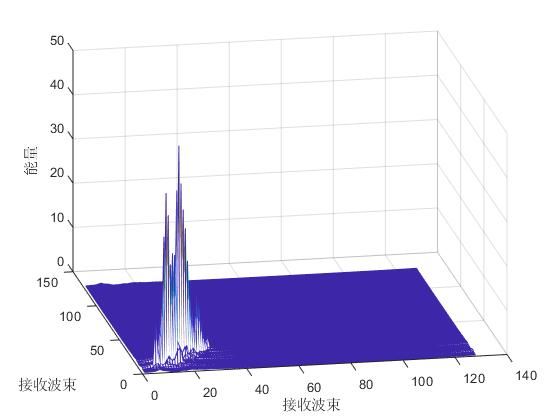
\includegraphics[width=0.6\textwidth]{img/2_4.jpg} \caption{用户多天线波束域信道基站侧相关阵}
\end{figure}


\section{本章小结}
本章主要研究了MIMO信道物理模型,统计模型和波束域信道模型。其中物理模型主要是研究了影响信道情况的各种参数,并为后续各种模型的基础。统计信道模型主要研究了联合相关模型,作为实际相关仿真模型的基础模型。波束域信道模型主要体现的是大规模MIMO信道的特性和研究方式,通过波束域信道模型的特征,提供了减少计算复杂度切入点。

\chapter{基于MMSE接收机复杂度优化}
\section{引言}
信号在通过上述复杂信道之后,信号会发生改变,此时需要利用一些判决方法将接收信号恢复为发送信号。但是因为通过信道后信号同样会收到随机干扰,所以完全恢复为初始信号某种意义上是不存在的,但是通过一些方法,可以尽可能地或者说最大概率的接近发送信号。这些根据接收信号恢复发送信号的方法在通信系统中称为检测,目前针对MIMO系统最佳的检测方法为MMSE估计。但是MMSE估计的计算复杂度随着天线的增多,信道矩阵维度的扩大,会变得非常高,实际系统实现会非常占用资源。而其主要复杂度主要来自于矩阵的求逆运算,而通过QR分解,可以将矩阵求逆运算化简为QR分解。QR分解的复杂度会比原始MMSE的复杂度大大降低。并且本文在信道模型重点描述了波束域信道,此时可以注意到波束域信道的信道是稀疏的,同样一定程度上减少了计算复杂度,本章的后续部分还会讨论空间域的MMSE以及复杂度优化
\section{系统模型}
在一个大规模MIMO系统中,一个基站将使用数以百计的天线来提供巨大的用户容量提高。在用户端,一般认为用户只有一根天线。但是,由于目前用户多天线的技术已经运用,将用户多天线应用到大规模MIMO系统中具有理论与实践的双重意义。所以在建立系统模型时,可以考虑用户多天线的情况。本文后续仿真将同时考虑用户单天线,用户多天线单流,用户多天线多流的情况。

考虑一个由一个基站(BS)和K个用户终端组成的系统,其中K个用户分别讨论其拥有单天线和多天线的情况。基站(BS)配有$N_R$根天线,第$k$个用户终端拥有$M_k$根天线,并且$\sum_{k=1}^K M_k = M$。考虑天线阵列为相隔为半波长$0.5\lambda$的线阵天线。根据上面的推导,可以得到基站第n根接收第i个用户的第r根的信号为
\begin{equation}\label{key}
r_{n,r} = \sum^{M_i}_{i=1} \sum_{p=1}^{P} \sum_{q=1}^{Q_p} \mathrm{Re} \left \lbrace u_{i,p,q} h_{p,q} (t) w_{i,p,q} s_b(t) e^{j 2\pi f_c t} \right \rbrace + n_{n,r}(t)
\end{equation}
其中,$h(t)$ 和 阵列响应如上。
\begin{eqnarray}\label{key}
h_{p,q}(t) = \alpha_{LNA}\beta\alpha_{PA}a_{p,q}e^{j(2\pi 
	(v_{p,q}t-v_{p,q}\tau_{p,q})+\phi_{p,q}
	)} \\
w_{n_{T},p,q} = \mathrm{exp}(-j2\pi \frac{d_{n_{T}}}{\lambda}\sin \theta_{p,q,AOD})\\
u_{n_{R},p,q} = \mathrm{exp}(-j2\pi \frac{d_{n_{R}}}{\lambda}\sin \theta_{p,q,AOA})
\end{eqnarray}
矩阵表达如下
\begin{eqnarray}\label{key}
\mathbf{r}_{i}(t) & = &[r_{1,i}(t) \quad r_{2,i}(t) \quad\dots\quad r_{N_{R},i}(t)]^{T} \\
\mathbf{x}_{i}(t)& = &[s_{1,i}(t) \quad s_{2,i}(t) \quad\dots\quad s_{N_{T},i}(t)]^{T} \\
\mathbf{n}_{i}(t)& = &[n_{1,i}(t) \quad n_{2,i}(t) \quad\dots\quad n_{N_{R},i}(t)]^{T} \\
\mathbf{H}_{i,p}(t)& = &\left[ \begin{array}{cccc}
h_{1,1,p}(t) & h_{1,2,p}(t) & \ldots & h_{1,M_{i},p}(t) \\
h_{2,1,p}(t) & h_{2,2,p}(t) & \ldots & h_{2,M_{i},p}(t) \\
\vdots & \vdots & \ddots & \vdots \\
h_{N_{R},1,p}(t) & h_{N_{R},2,p}(t) & \ldots & h_{N_{R},M_{i},p}(t)
\end{array} \right] 
\end{eqnarray}
由上面的矩阵表达和信号的物理表达式,可以将基带信号建模为
\begin{equation}\label{key}
\mathbf{r}_{i}(t) = \sum_{p=1}^{P}\mathbf{H}_{i,p}(t)\mathbf{x}_{i}(t) + \mathbf{n}_{i}(t)
\end{equation}
本文在这里将信道模型简写为
\begin{equation}\label{key}
\mathbf{y} = \sum_{i=1}^{K} \mathbf{H}_i \mathbf{x}_i + \mathbf{Z}
\end{equation}
考虑带宽为B,零均值,协方差矩阵为$\sigma^{2}\mathbf{I}_{M_{r}}$的噪声,$\sigma^{2} \triangleq \mathbb{E}[n^{2}_{i}]= N_{0}/2$。并有发射信号
\begin{equation}\label{key}
\sum_{i=1}^{M_{t}}\mathbb{E}[x_{i}x_{i}^{*}] = P
\end{equation}
或者可以写为
\begin{equation}\label{key}
\mathbb{E}[\mathrm{tr}(\mathbf{x}\mathbf{x}^{H})] = P
\end{equation}
则信道矩阵有
\begin{equation}\label{key}
\mathbb{E}[\mathrm{tr}(\mathbf{H}\mathbf{H}^{H})] = N_{R}N_{T}
\end{equation}
发射功率约束$P$将根据$P/\sigma^{2} = \rho$得到SNR$\rho$,同时如果考虑天线能量均匀分布的话有$\mathbb{E}[(\mathbf{x}\mathbf{x}^{H})] = (P/N_{t})I_{N_{t}} $,$\rho$可以用来表示在单通道增益下单根接收天线的平均信噪比SNR。为了简化模型,有时会将噪声功率归一化,此时$\rho$也可以用来表示发射功率。
同样可以改写性质为下
\begin{equation}\label{key}
\mathbb{E} \lbrace \mathrm{tr} (\mathbf{H}_i \mathbf{H}_i^H ) \rbrace = \frac{N M_i}{M}
\end{equation}
根据此性质$\mathbb{E} \lbrace \mathrm{tr} (\mathbf{H}_i \mathbf{H}_i^H ) \rbrace = \frac{N M_k}{M}$,本文可以套用联合相关信道模型
\begin{eqnarray}\label{key}
\mathbf{H}_i & = & \mathbf{U}_{r}\tilde{\mathbf{H}}\mathbf{U}_{t}^{H} = \mathbf{U}_{r}(\mathbf{D}+\mathbf{M}_i\odot \mathbf{H}_{idd})\mathbf{U}_{t}^{H} \\ \nonumber
& = & \mathbf{U}_{r}\mathbf{D}\mathbf{U}_{t}^{H} + \mathbf{U}_{r}(\mathbf{M}\odot \mathbf{H}_{idd})\mathbf{U}_{t}^{H}\mathbf{U}_{t}^{H}
\end{eqnarray}
其中$U_r$和$U_t$以及其他符号均与上面推导的式子相同,此处本文为了方便后续计算将$\mathbf{H}_{idd}$的方差设为$\frac{1}{M}$。
令
\begin{gather}\label{key}
\overline{\mathbf{H}}_i = \mathbf{U}_{r}\mathbf{D}\mathbf{U}_{t}^{H} \\
\tilde{\mathbf{H}}_i = \mathbf{U}_{r}(\mathbf{M}_i\odot \mathbf{H}_{idd})\mathbf{U}_{t}^{H}\mathbf{U}_{t}^{H}
\end{gather}
根据性质,可以得出结论
\begin{equation}\label{key}
\mathbb{E} \lbrace \tilde{\mathbf{H}}_i \mathbf{C}_{ij} \tilde{\mathbf{H}}_j^{H} \rbrace = 0_{N*N}
\end{equation}
\begin{equation}\label{key}
\mathbb{E} \lbrace \tilde{\mathbf{H}}_i^{H} \tilde{\mathbf{C}}_{ij} \tilde{\mathbf{H}}_j \rbrace = 0_{M_i*M_j}
\end{equation}
其中,$\mathbf{C}_{ij}$是一个$M_i \times M_j$ 维的常数矩阵,$\tilde{\mathbf{C}}_{ij}$ 是一个$N \times N$维的常数矩阵
类似上面统计信道,定义能量耦合矩阵为
\begin{equation}\label{key}
\bm{\Omega} =\mathbb{E}[\tilde{\mathbf{H}} \odot \tilde{\mathbf{H}}^{*}]
\end{equation}
即
\begin{equation}\label{key}
\bm{\Omega} =\mathbf{M_i} \odot \mathbf{M}
\end{equation}
则可以写出信道的单边相关矩阵$\tilde{\eta}_i$表达式
\begin{equation}\label{key}
\tilde{\eta}_i = \mathbb{E} \lbrace \tilde{\mathbf{H}}_i \mathbf{C}_i \tilde{\mathbf{H}}_i^H \rbrace
\end{equation}
并有
\begin{equation}\label{key}
{\eta}_i = \mathbb{E} \lbrace \tilde{\mathbf{H}}_i^H \mathbf{C}_i \tilde{\mathbf{H}}_i \rbrace
\end{equation}
根据上面的波束域模型推导和统计信道模型令矩阵$\tilde{\Pi}_i$为$N \times N$的对角矩阵
\begin{equation}\label{key}
\tilde{\Pi}_i = \sum_{j=1}^{M_i}[\bf{\Omega}]_{ij}  [\mathbf{U}_t^H \mathbf{C}_i \mathbf{U}_t]_{jj}
\end{equation}
则有
\begin{equation}\label{key}
\tilde{\eta}_i = \mathbf{U}_r \tilde{\Pi}_i \mathbf{U}_r^H
\end{equation}



\section{MMSE接收机原理及仿真}
MMSE估计是最小均放误差估计的缩写,其判决准则如下式
\begin{equation}\label{key}
\hat{x}_{MMSE}(y) = \arg \min \mathbb{E}[\| x - \hat{x} \|^{2}]
\end{equation}
根据期望的性质以及复矢量微分和复矩阵微分,要使误差最小对$\hat{x}^{*}$方向求梯度为0即可以得到
\begin{equation}\label{key}
\hat{x}_{MMSE}(y) = \mathbb{E}[x|y]
\end{equation}
考虑线性最小均方误差,可以得出线性表达式
\begin{equation}\label{key}
\hat{x}_{LMMSE}(y)=\mathbf{W}y+b
\end{equation}
同一般情况的MMSE一致,线性最小均方误差是对$W^{*}$和$b^{*}$方向求梯度为0,以及设置在高斯白噪声信道下可以得到
\begin{equation}\label{key}
\left\{
\begin{array}{l}
\mathbf{W}=C_{x}\mathbf{H}^{H}(\mathbf{H}C_{x}\mathbf{H}^{H} + \sigma^{2}I)^{-1} \\
b=\mathbb{E}[x] - C_{x}\mathbf{H}^{H}(\mathbf{H}C_{x}\mathbf{H}^{H} + \sigma^{2}I)^{-1}\mathbf{H}\mathbb{E}[x]
\end{array}
\right.
\end{equation}
带入可得线性最小均方误差表达式
\begin{equation}\label{key}
\hat{x}_{LMSSE}(y)=\mathbb{E}[x]+C_{x}\mathbf{H}^{H}(\mathbf{H}C_{x}\mathbf{H}^{H}+\sigma^{2}I)^{-1}(y-\mathbf{H}\mathbb{E}[x])
\end{equation}
根据条件高斯PDF推导可得
\begin{equation}\label{key}
\mathbb{E}[x|y]=\mu_{x}+C_{xy}C_{yy}^{-1}(y-\mathbb{E}[y])
\end{equation}
\begin{equation}\label{key}
C_{x|y} = C_{xx} -C_{xy}C_{yy}^{-1}C_{yx}
\end{equation}
根据发送信号均值和接收信号均值,以及协方差矩阵可以得到
\begin{equation}\label{key}
\mathbb{E}[x|y]=\mu_{x} + C_{x}\mathbf{H}^{H}(\mathbf{H}C_{x}\mathbf{H}^{H}+\sigma^{2}I)^{-1}(y-\mathbf{H}\mu_{x})
\end{equation}
\begin{equation}\label{key}
C_{x|y}=C_{x}-C_{x}\mathbf{H}^{H}(\mathbf{H}C_{x}\mathbf{H}^{H}+\sigma^{2}I)^{-1}\mathbf{H}C_{x}
\end{equation}
根据矩阵求逆定理
\begin{equation}\label{key}
(A + BCD)^{-1} = A^{-1} - A^{-1}B(DA^{-1}B+C^{-1})^{-1}DA^{-1}
\end{equation}
根据上式,可以将式(3.29)和(3.30)转换成如下形式
\begin{gather}\label{key}
\mathbb{E}[x|y] = \mu_{x} + (\mathbf{H}C_n^{-1}\mathbf{H}^H + C_x^{-1})^{-1}\mathbf{H}^H C_n^{-1}(y-\mathbf{H}\mu_{x}) \\ 
C_{x|y} = (\mathbf{H} C_n^{-1} \mathbf{H}^H + C_x^{-1})^{-1}
\end{gather}
根据式(3.24)可以知道,且一般情况下,二进制采样后的信号均值为0,则MMSE的检测矩阵为
\begin{equation}\label{key}
\mathbf{W} = ({\mathbf{H}}{\mathbf{H}}^H + \sigma^2 {I})^{-1}{\mathbf{H}}^H
\end{equation}
同时得到MMSE准则计算公式
\begin{equation}\label{key}
\hat{x}_{MMSE} = (\mathbf{H}\mathbf{H}^H + \sigma^2 I)^{-1}\mathbf{H}^\mathbf{H} y
\end{equation}
而代入上述系统模型,则上式应写作
\begin{equation}\label{key}
\hat{\mathbf{x}}_{MMSE} = (\mathbf{H}\mathbf{H}^H + \sigma^2 \mathbf{I})^{-1}\mathbf{H}^H \mathbf{y}
\end{equation}
其中$\mathbf{H}$代表$[\mathbf{H}_1,\mathbf{H}_2,...,\mathbf{H}_K]$,令$\mathbf{x}$代表$[\mathbf{x}_1^T,\mathbf{x}_2^T,...,\mathbf{x}_K^T]$


根据MMSE估计,本文做了MMSE估计的仿真,并以MMSE估计作为评判基准,此处考虑的为BPSK调制。分别考虑用户单天线和用户多天线,多天线时设置为2和4。判决采用硬判决,即判断不会受到前后判决结果的影响,在用户多天线单流的情况下,判决结果会按照多天线取平均。
\begin{table}[htbp]
	\centering
	\caption{\label{tab:test}MMSE仿真参数设置}
	\begin{tabular}{ll}
		\toprule
		参数 &  设置值 \\
		\bottomrule
		场景 &  郊区宏蜂窝 \\
		\bottomrule
		基站侧天线数 & 128 \\
		\bottomrule
		用户数天线	& 1 \quad or\quad2 \\
		\bottomrule
		用户数	& 4 \\
		\bottomrule
		天线间距 & 0.5$\lambda$ \\
		\bottomrule
		路径数 & 6 \\
		\bottomrule
		用户采样数量 & 10000 \\
		\bottomrule
	\end{tabular}
\end{table}

\begin{figure}[htbp!]
	\centering 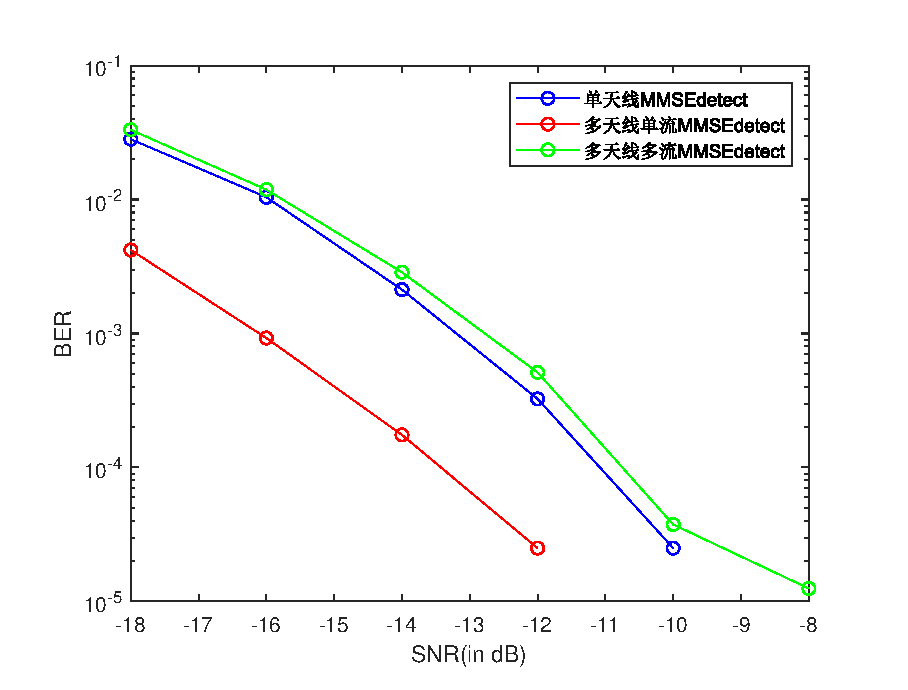
\includegraphics[width=0.7\textwidth]{img/3_8.eps} \caption{MMSE检测BER}
\end{figure}

从图3.1,可以看出对于不同的情况即用户单天线,用户多天线单流,用户多天线多流的情况各不相同。其中多天线单流应是判断准确度最高,其次为用户单天线,其次用户多天线多流。其中多天线单流,因为多天线传输的相同的数据能够通过综合所得到的数据得出最好的结果,而用户单天线与用户多天线多流的不同在于多天线多流带来了天线与天线之间的干扰,导致判断准确度下降。本文将主要从这三种情况对本文提出的低复杂度算法进行分析研究。而上述的MMSE模型将作为判断低复杂度算法是否达标的基准。


\section{QR分解方法}
虽然可以通过上式,很容易得到MMSE的检测矩阵的表达式,但需要注意的是信道矩阵$\mathbf{H}$是一个维度相对较大的矩阵,所以上式计算是非常困难的。并且在FPGA等硬件上实现矩阵求逆转置是比较繁琐的,所以通常MMSE矩阵硬件上实现是以QR分解为基础进行计算,其复杂度一定程度上得到简化。
下面简单介绍QR分解,即将信道矩阵分解为Q阵和R阵,其中Q阵为正交阵,R阵为上三角矩阵
令
\begin{equation}\label{key}
\overline{\mathbf{H}} = \left[
\begin{array}{c}
\mathbf{H}\\
\sigma \mathbf{I}
\end{array} \right] =
\left[
\begin{array}{c}
\mathbf{Q}_1\\
\mathbf{Q}_2
\end{array} \right] \mathbf{R}
\end{equation}
根据MMSE检测计算公式
\begin{equation}\label{key}
\hat{x}_{MMSE} = (\mathbf{H}\mathbf{H}^H + \sigma^2 \mathbf{I})^{-1}\mathbf{H}^H y
\end{equation}
有
\begin{equation}\label{key}
\mathbf{W}=(\overline{\mathbf{H}}^H \overline{\mathbf{H}})^{-1} \mathbf{H}^H
\end{equation}
\begin{equation}\label{key}
\mathbf{H} = \mathbf{Q}_1 \mathbf{R} ,\sigma\mathbf{I} = \mathbf{Q}_2\mathbf{R}
\end{equation}
又因为$\mathbf{Q}_1,\mathbf{Q}_2$是正交阵
\begin{equation}\label{key}
\mathbf{R} = \sigma \mathbf{Q}_2^{-1}
\end{equation}
\begin{equation}\label{key}
(\overline{\mathbf{H}}^H \overline{\mathbf{H}})^{-1} = (\mathbf{R}^H \mathbf{Q}^H\mathbf{Q} \mathbf{R})^{-1} =(\mathbf{R}^H \mathbf{R})^{-1}
\end{equation}
又有
\begin{equation}\label{key}
\mathbf{H}^{H} =\mathbf{R}^{H} \mathbf{Q}_1^H 
\end{equation}
所以式(3.39)有
\begin{equation}\label{key}
\mathbf{W} = \mathbf{R}^{-1} \mathbf{Q}_1^H
\end{equation}
由此可以容易得到检测矩阵的表达式为
\begin{equation}\label{key}
\mathbf{W}=(\overline{\mathbf{H}}^H \overline{\mathbf{H}})^{-1} \mathbf{H}^H = \frac{1}{\sigma} \mathbf{Q}_2 \mathbf{Q}_1^H
\end{equation}

下面本文简单介绍一下常用的QR分解的方法,一般使用QR分解可以用下面三种方法来完成,Gram-Schmit正交化QR分解,Givens矩阵与Givens旋转,Householder矩阵与Householder变换。上面三个不同的QR分解适合不同的系统模型,或者是指不同的情况下。
Gram-Schmit正交化适用于满秩矩阵,当$\mathbf{H}$为满秩矩阵时,$\overline{\mathbf{H}}$也是一个满秩矩阵。将$\overline{\mathbf{H}}$写为$[\alpha_1^T \alpha_2^T ... \alpha_n^T]$形式,
令
\begin{eqnarray}\label{key}
\beta_1 = \alpha_1 , \beta_2 = \alpha_2 - k\beta_1 , k = \frac{<\alpha_2,\beta_1>}{<\beta_1,\beta_1>} \nonumber
\end{eqnarray}
依次类推,则有
\begin{equation}\label{key}
\beta_i = \alpha_i - k_1\beta_1 -k_2\beta_2 - ... - k_{i-1}\beta_{i-1} \nonumber
\end{equation}
\begin{equation}\label{key}
k_j = \frac{<\alpha_i,\beta_j>}{<\beta_j,\beta_j>}, j= 1,2,3,...,i \nonumber
\end{equation}
从而,得到的$\mathbf{Q}$矩阵可令其为$[\beta_1^T,\beta_2^T,...,\beta_n^T]$,$\mathbf{Q}$矩阵是正交阵,$\mathbf{R}$矩阵是$\overline{\mathbf{H}}$到$\mathbf{R}$的变换矩阵。\\

Givens旋转主要是利用Givens矩阵的旋转特性去计算上三角阵$\mathbf{R}$而多个Givens矩阵的乘法和矩阵$\mathbf{G}_1...\mathbf{G}_n$根据Givens矩阵的特性也满足要求,为正交阵。
\begin{eqnarray}\label{key}
G(i,j,\theta) = \left[
\begin{array}{ccccccc}
1 & \ldots & 0 & \ldots & 0 & \ldots & 0 \\
\vdots & \ddots & \vdots & \quad & \vdots & \quad & \vdots \\
0 & \ldots & c & \ldots & s & \ldots & 0 \\
\vdots & \quad & \vdots & \ddots & \vdots & \quad & \vdots \\
0 & \ldots & -s & \ldots & c & \ldots & 0 \\
\vdots & \quad & \vdots & \quad & \vdots & \ddots & \vdots \\
0 & \ldots & 0 & \ldots & 0 & \ldots & 1 
\end{array}
\right]
\end{eqnarray}
$c=\cos\theta$ 和 $s = \sin\theta$ 出现在第i行和第j行与第i列和第j列的交叉点上,亦可以这样描述Givens矩阵的非零元素
\begin{gather}\label{key}
g_{kk} = 1 , \quad k \neq i,j  \nonumber\\ 
g_{ii} = c  \nonumber \\
g_{jj} = c  \nonumber \\
g_{ij} = s  \nonumber \\
g_{ji} = -s  \nonumber \\  
c=\cos\theta  \nonumber \\
s = \sin\theta  \nonumber
\end{gather}
主要是对目标矩阵的第i行和第j行进行变换。QR分解的Givens变换是为了将部分元素变换为0,即
\begin{eqnarray}\label{key}
\left[
\begin{array}{ccccccc}
1 & \ldots & 0 & \ldots & 0 & \ldots & 0 \\
\vdots & \ddots & \vdots & \quad & \vdots & \quad & \vdots \\
0 & \ldots & c & \ldots & s & \ldots & 0 \\
\vdots & \quad & \vdots & \ddots & \vdots & \quad & \vdots \\
0 & \ldots & -s & \ldots & c & \ldots & 0 \\
\vdots & \quad & \vdots & \quad & \vdots & \ddots & \vdots \\
0 & \ldots & 0 & \ldots & 0 & \ldots & 1 
\end{array}
\right]
\left[
\begin{array}{c}
x \\
\vdots \\
\alpha \\
\vdots \\
\beta \\
\vdots  \\
x
\end{array}
\right]
=\left[
\begin{array}{c}
x \\
\vdots \\
\gamma \\
\vdots \\
0 \\
\vdots  \\
x
\end{array}
\right]
\end{eqnarray}
即
\begin{equation}\label{key}
c = \frac{\alpha}{\sqrt{\alpha^2+\beta^2}}
\end{equation}
\begin{equation}\label{key}
s =\frac{\beta}{\sqrt{\alpha^2+\beta^2}}
\end{equation}
而类似(3.42),QR分解MMSE检测矩阵就是将$\mathbf{W}$看作列向量的结合,将向量按照从下至上依次转置为0,即
\begin{eqnarray}\label{key}
\left[
\begin{array}{cccccc}
1 & \ldots & 0 &  0 & \ldots & 0 \\
\vdots & \ddots & \vdots &  \vdots & \quad & \vdots \\
0 & \ldots & c &  s & \ldots & 0 \\
0 & \ldots & -s &  c & \ldots & 0 \\
\vdots & \quad & \vdots &  \vdots & \ddots & \vdots \\
0 & \ldots & 0 &  0 & \ldots & 1 
\end{array}
\right]
\left[
\begin{array}{ccc}
x_{11} & \ldots & x_{1n} \\
\vdots & \ldots & x_{pn}\\
\alpha & \ldots & x_{qn}\\
\beta& \ldots & x_{rn} \\
\vdots  & \ldots & x_{tn}\\
0& \ldots & x_{sn}
\end{array}
\right]
=\left[
\begin{array}{ccc}
x_{11}' & \ldots & x_{1n}'\\
\vdots & \ldots & x_{pn}'\\
\gamma & \ldots & x_{qn}'\\
0 & \ldots & x_{rn}'\\
\vdots  & \ldots & x_{tn}'\\
0& \ldots & x_{sn}'
\end{array}
\right]
\end{eqnarray}
通过$n*n/2$次Givens旋转,可以得到一个上三角阵,而Givens矩阵的乘积即为Q阵。\\

Householder变换主要是利用Householder矩阵将$\overline{\mathbf{H}}$特定位置的值转换为0,即求解$\overline{\mathbf{H}}$的上三角阵$\mathbf{R}$。Householder矩阵对一个向量的表达式如下
\begin{equation}\label{key}
\mathbf{H} = \mathbf{I} - \frac{2}{<\mathbf{v},\mathbf{v}>} \mathbf{v}\mathbf{v}^H
\end{equation}
即分别对$\overline{\mathbf{H}}$每列进行Householder变化将其变换为上三角正,而Householder矩阵的乘积和即为QR分解的$\mathbf{Q}$阵。
Householder矩阵是对称矩阵,正交矩阵,Hermitian矩阵,对合矩阵
\begin{gather}\label{key}
\mathbf{H}^T = \mathbf{H}  \nonumber \\
\mathbf{H}^T = \mathbf{H}^{-1}  \nonumber\\
\mathbf{H}^H = \mathbf{H}  \nonumber\\
\mathbf{H}^2 = \mathbf{I} \nonumber
\end{gather}
即可以根据$\mathbf{H}^H\mathbf{H}=\mathbf{I}$得到$\mathbf{v}\mathbf{v}^H =\mathbf{I}$
而Householder变换可以将矩阵变换到$\mathbf{v}$向量代表的坐标轴的投影。即
\begin{equation}\label{key}
\mathbf{H}\mathbf{x} =\alpha [1 \quad 0 \quad \ldots 0]^T
\end{equation}
令$\mathbf{e}_1=[1 \quad 0 \quad \ldots 0]^T$,
根据Householder矩阵的定义,可以得到
\begin{equation}\label{key}
\frac{1}{2}(\mathbf{x}-\alpha \mathbf{e}_1)=(\mathbf{v}^H\mathbf{x})\mathbf{v}
\end{equation}
其中每一个$\mathbf{v}$向量中的元素可以如下定义
\begin{eqnarray}\label{key}
v_1 & = & \frac{x_1-\alpha}{\| \mathbf{x} - \alpha \mathbf{e}_1 \|_2} \nonumber \\
& = & -\frac{\alpha-x_1}{\sqrt{2\alpha(\alpha-x_1)}} \nonumber \\
v_2 & = & \frac{x_2}{2\alpha v_1} \nonumber  \\
\vdots \nonumber \\
v_n & = & \frac{x_n}{2\alpha v_1}
\end{eqnarray}
利用Householder变换求解QR分解的步骤大致如下,下面用$\mathbf{P}^{(n)}$表示第n个Householder矩阵。目标矩阵写为
\begin{eqnarray}\label{key}
\mathbf{H}^{(i)} =
\left[
\begin{array}{ccccccc}
x_{11} & \ldots & x_{1i} & \ldots & x_{1j} & \ldots & x_{1k} \\
\vdots & \ddots & \vdots & \quad & \vdots & \quad & \vdots \\
0 & \ldots & x_{pi} & \ldots & x_{pj} & \ldots & x_{pk} \\
\vdots & \quad & \vdots & \ddots & \vdots & \quad & \vdots \\
0 & \ldots & x_{qi} & \ldots & x_{qj} & \ldots & x_{qk} \\
\vdots & \quad & \vdots & \quad & \vdots & \ddots & \vdots \\
0 & \ldots & x_{ni} & \ldots & x_{nj} & \ldots & x_{nk} 
\end{array}
\right]
\end{eqnarray}
对i列进行处理,即选取i列的$i+1 ~ n$个元素,用$S$代替,得到第i个Householder矩阵$\mathbf{P}^{(i)}$,即
\begin{equation}\label{key}
\mathbf{P}^{(i)} \S = [1 \quad 0 \quad \ldots 0]^T
\end{equation}
即
\begin{equation}\label{key}
\mathbf{P}^{(i)}\mathbf{H}^{(i)} =\mathbf{P}^{(i)}
\left[
\begin{array}{ccccccc}
x_{11} & \ldots & x_{1i} & \ldots & x_{1j} & \ldots & x_{1k} \\
\vdots & \ddots & \vdots & \quad & \vdots & \quad & \vdots \\
0 & \ldots & x_{pi} & \ldots & x_{pj} & \ldots & x_{pk} \\
\vdots & \quad & \vdots & \ddots & \vdots & \quad & \vdots \\
0 & \ldots & x_{qi} & \ldots & x_{qj} & \ldots & x_{qk} \\
\vdots & \quad & \vdots & \quad & \vdots & \ddots & \vdots \\
0 & \ldots & x_{ni} & \ldots & x_{nj} & \ldots & x_{nk} 
\end{array}
\right]
= 
\left[
\begin{array}{ccccccc}
x_{11} & \ldots & x_{1i} & \ldots & x_{1j} & \ldots & x_{1k} \\
\vdots & \ddots & \vdots & \quad & \vdots & \quad & \vdots \\
0 & \ldots & x_{ii} & \ldots & x_{ij} & \ldots & x_{ik} \\
\vdots & \quad & \vdots & \ddots & \vdots & \quad & \vdots \\
0 & \ldots & 0 & \ldots & x_{qj} & \ldots & x_{qk} \\
\vdots & \quad & \vdots & \quad & \vdots & \ddots & \vdots \\
0 & \ldots & 0 & \ldots & x_{nj} & \ldots & x_{nk} 
\end{array}
\right]
\end{equation}
这个过程总共只需要进行n次即可以得到上三角阵$\mathbf{R}$,而变换矩阵的乘积即为正交矩阵$\mathbf{Q}$。

从本文上面所写的一般的MMSE复杂度主要是信道矩阵的求逆带来的,普通MMSE的复杂度为$\Theta(M^3)$。如果采用QR分解优化的MMSE的计算,采用不同的QR分解有不同的复杂度。Gram-Schmit正交化QR分解和Givens变换QR分解的计算复杂度在计算一般信道矩阵时仍为$\Theta(M^3)$。而Householder变换的计算复杂度为$\Theta(M^2)$。对于一般情况的信道矩阵时,Givens旋转计算复杂度并不会比普通的MMSE减少很多,但Givens旋转由于其矩阵的特定形式,可以只改变旋转的i行i列和j行j列,所以可以利用这个性质,对MMSE进行并行计算,从而降低MMSE检测的时间,但是计算复杂度上并不会减少。
由于QR分解计算MMSE是有严格数学推导的,所以所得到的结果应该与MMSE检测的结果一致。

但是,可以注意到的是当矩阵稀疏时,Givens变换的计算复杂度就会降低。而推导QR分解使用矩阵
\begin{equation}\label{key}
\overline{\mathbf{H}} = \left[
\begin{array}{c}
\mathbf{H}\\
\sigma \mathbf{I}
\end{array} \right]
\end{equation}
其下半部分属于单位阵,所以在并行计算的同时,Givens变换的复杂度同样降低了n次操作,所以此时的Givens变换的计算复杂度同样为$\Theta(M^2)$,但是考虑到这里的矩阵是被扩充过的,所以先对与原始MMSE并不会有很大程度的降低。
而由本文上面提到的波束域信道模型,当物理信道乘以信道矩阵的特征矩阵时,此时为波束域信道,不仅扩充部分稀疏,信道矩阵也为稀疏阵,此时使用Givens变换和Householder变换的复杂度将会进一步的降低。但是在一般的信道矩阵,因为接收天线的数量不能逼近无穷大,按照一般公式无法计算出严格稀疏的信道矩阵,而讨论的降低复杂度需要稀疏矩阵。所以这里进行了近似处理,将相对较小的元素直接赋值为0。这必然会带来一定的误差,而接下来的部分,将利用仿真结果去判断。
\begin{figure}[htbp!]
	\centering 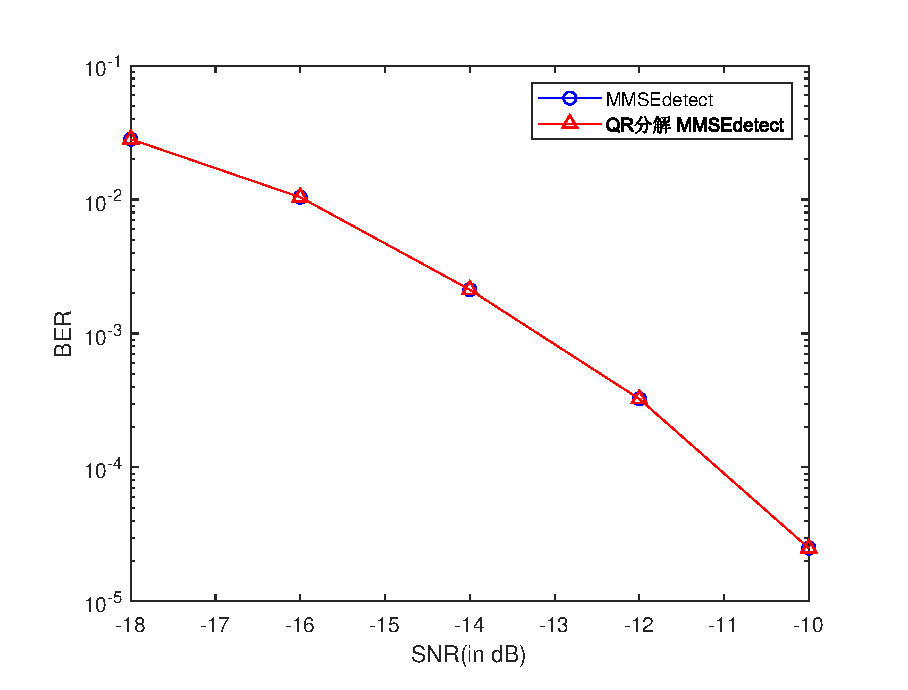
\includegraphics[width=0.5\textwidth]{img/3_9.eps} \caption{QR分解MMSE}
\end{figure}

\section{低复杂度的MMSE接收机}
本文第二章论证的波束域信道矩阵有这样的性质,波束域信道矩阵的不同列代表着不同的接收角,又称为波束。而通过第二章基站侧信道矩阵得到的相关阵和能量耦合矩阵,可以得到对于单个用户来说,其所使用的波束数量是有限且比较少的,所以使用波束域信道矩阵时可以发现波束域信道矩阵是稀疏的。而稀疏的信道矩阵在进行计算时可以利用很多种方法进行优化复杂度。这里本文考虑的是严格的数学推导得到QR分解,对于稀疏阵的计算可以通过更多方式进行化简。
根据第二章,本文有
\begin{equation}\label{key}
\mathbf{H}_{F} = \mathbf{F} \mathbf{H}
\end{equation}
可以得到波束域信道,假定信号传播在波束域,那么信号通过的应是波束域信道,但是真实情况是信号传输在物理信道中,所以需要在判决时的接收信号前乘上DFT矩阵使其同样处于波束域。即
\begin{equation}\label{key}
\mathbf{y}_F =\mathbf{F} \mathbf{y}
\end{equation}
从而得到波束域信道下MMSE矩阵
\begin{equation}\label{key}
\hat{\mathbf{x}}_{MMSE} = (\mathbf{H}_F\mathbf{H}_F^H + \sigma^2 \mathbf{I})^{-1}\mathbf{H}_F^H \mathbf{y}_F
\end{equation}
其中$\mathbf{H}_F$代表$[\mathbf{F}\mathbf{H}_1,\mathbf{F}\mathbf{H}_2,...,\mathbf{F}\mathbf{H}_K]$,令$\mathbf{x}$代表$[\mathbf{x}_1^T,\mathbf{x}_2^T,...,\mathbf{x}_K^T]$
通过第二章的理论推导,可以知道严格稀疏是建立在基站天线数量趋近于$\infty$,但是本文所使用的模型基站天线存在数量限制,所以需要一些近似处理,将信道矩阵处理为严格稀疏,从而适应低复杂度的算法,此处可能会出现一些误差,本文主要分析利用这样的近似处理是否会影响检测结果。
由图3.5,可知原始信道矩阵并不是稀疏的。所以本文提出波束域的降低复杂度方法在原始信道矩阵并不起作用,同时经过式(3.60)的处理后,可以发现波束域信道矩阵此时是有稀疏矩阵的趋势,但是由于天线数的限制,所以本文做了近似处理,即设置门限值,将低于门限值的波束域信道矩阵元素赋值为零,此时波束域信道矩阵严格稀疏
\begin{equation}\label{key}
if\quad [\mathbf{H}_F]_{ij} <\lambda \quad then \quad [\mathbf{H}_F]_{ij}=0;
\end{equation}
本文采用的门限值为0.5,通过不同的门限值选择可能会影响矩阵的稀疏程度,同样的也会影响准确度和计算复杂度。经过近似处理后的信道如图3.7,可以看出严格稀疏波束域信道与原始信道区别并不大。
所以令
\begin{equation}\label{key}
\mathbf{H}_{approx} \approx \mathbf{H}_F
\end{equation}
带入MMSE判决公式
\begin{equation}\label{key}
\hat{\mathbf{x}}_{approx\quad MMSE} = (\mathbf{H}_{approx}\mathbf{H}_{approx}^H + \sigma^2 \mathbf{I})^{-1}\mathbf{H}_{approx}^H \mathbf{y}_F
\end{equation}
此时上式利用QR分解计算MMSE的复杂度,上文提到了使用Givens变换的QR分解需要对目标矩阵下三角区每一个非零元素进行QR变换,而此时的信道矩阵严格稀疏,则需要进行的Givens变换将会减少,由此可以推知复杂度与用户的所占波束相关,复杂度为$\Theta((N_u*N_{beam})^2)$。

\begin{figure}[htbp!]
	\centering 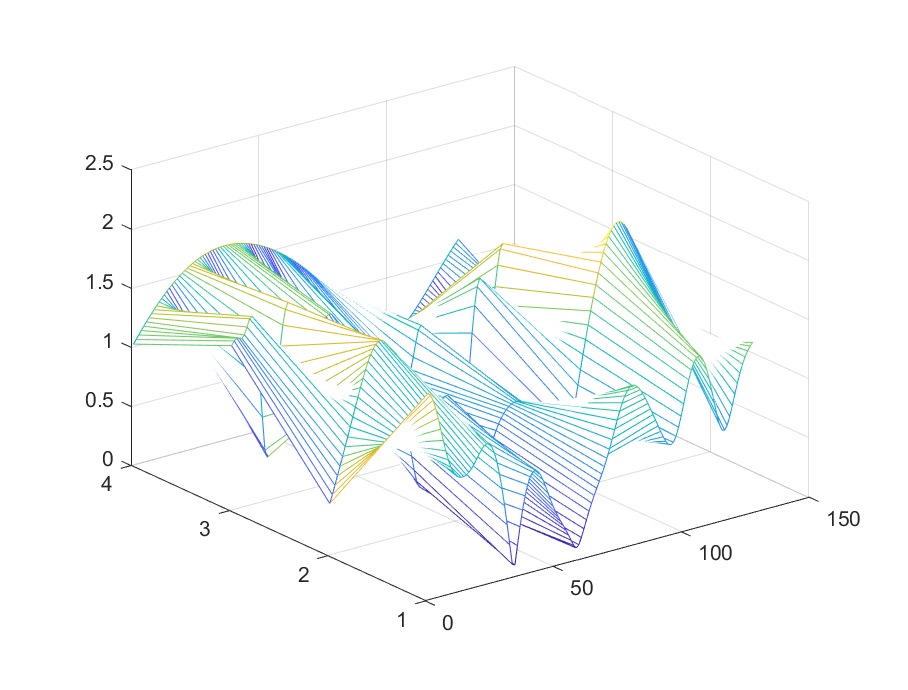
\includegraphics[width=0.45\textwidth]{img/3_1.eps} \caption{原始信道矩阵}
\end{figure}
\begin{figure}[htbp!]
	\centering 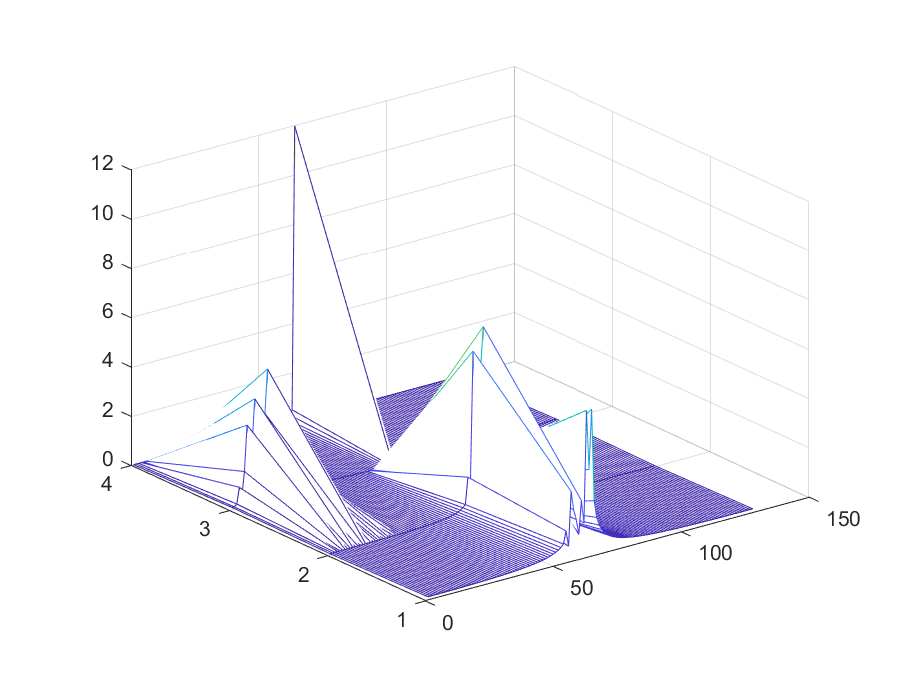
\includegraphics[width=0.45\textwidth]{img/3_2.eps} \caption{原始波束域信道矩阵}
\end{figure}
\begin{figure}[htbp!]
	\centering 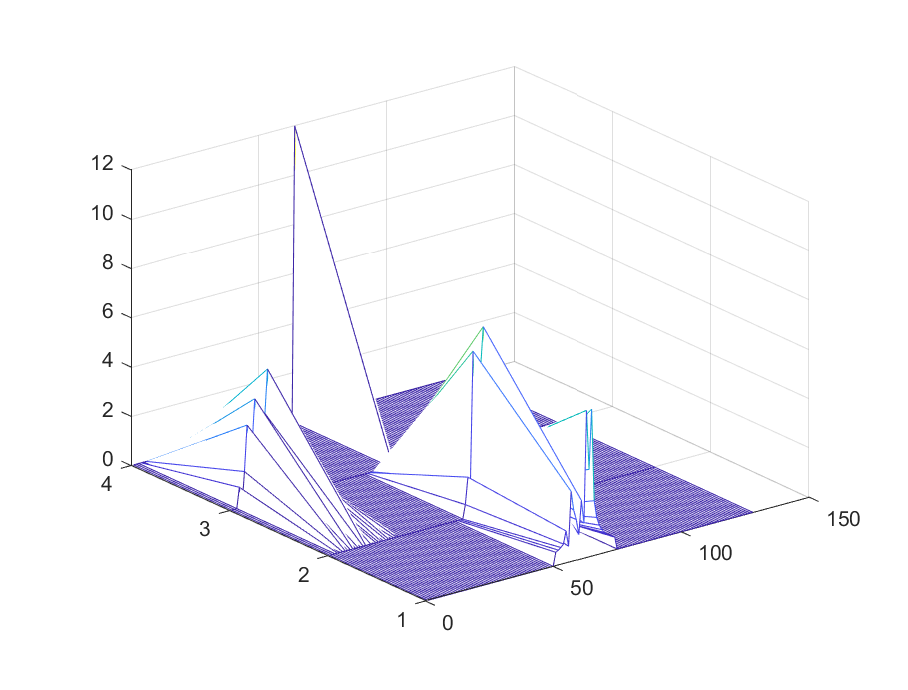
\includegraphics[width=0.45\textwidth]{img/3_3.eps} \caption{近似处理波束域信道矩阵}
\end{figure}
下面本文将具体讨论利用波束域信道的低复杂度MMSE接收机的表现
类似的测试情况为BPSK调制无编码。分别考虑用户单天线和用户多天线,多天线时设置为2和4。判决采用硬判决,即判断不会受到前后判决结果的影响,在用户多天线单流的情况下,判决结果会按照多天线取平均。
\begin{table}[htbp]
	\centering
	\caption{\label{tab:test}低复杂度MMSE仿真参数设置}
	\begin{tabular}{ll}
		\toprule
		参数 &  设置值 \\
		\bottomrule
		场景 &  郊区宏蜂窝 \\
		\bottomrule
		基站侧天线数 & 128 \\
		\bottomrule
		用户数天线	& 1 \quad or\quad 2 \quad  or\quad4\\
		\bottomrule
		用户数	& 4 \\
		\bottomrule
		天线间距 & 0.5$\lambda$ \\
		\bottomrule
		路径数 & 6 \\
		\bottomrule
		用户采样数量 & 10000 \\
		\bottomrule
	\end{tabular}
\end{table}

从图3.8,3.9,3.10,3.11来看利用QR分解以及波束域特性的低复杂度MMSE的检测方式性能和普通MMSE检测方式几乎没有区别,在上述提到的四种情况都有非常好的逼近普通MMSE。此低复杂度MMSE检测方式性能上基本符合要求,而且根据前面的推导,也可知该接收机很大程度上还是降低的复杂度。根据结果,还是可以发现当用户的天线数增多之后,低复杂度的MMSE的性能还是略微低于普通MMSE。原因可能是多天线所占用的波束较多,并且能量较多的几个波束占用总共接收能量的比例有所下降,导致检测性能下降。通过调整上面所设置的门限值$\lambda$可以缩小波束域低复杂度MMSE和普通MMSE的差距。同样的,调整$\lambda$也可以将准确度换取更低的计算复杂度。

\begin{figure}[htbp!]
	\centering 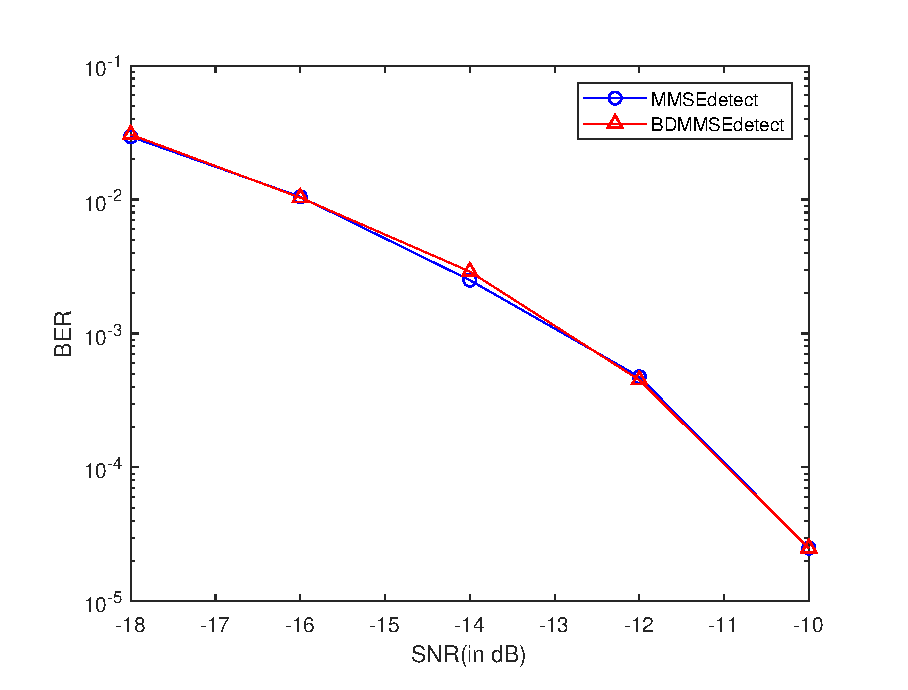
\includegraphics[width=0.55\textwidth]{img/3_4.eps} \caption{4用户单天线普通MMSE与波束域MMSE对比}
\end{figure}
\begin{figure}[htbp!]
	\centering 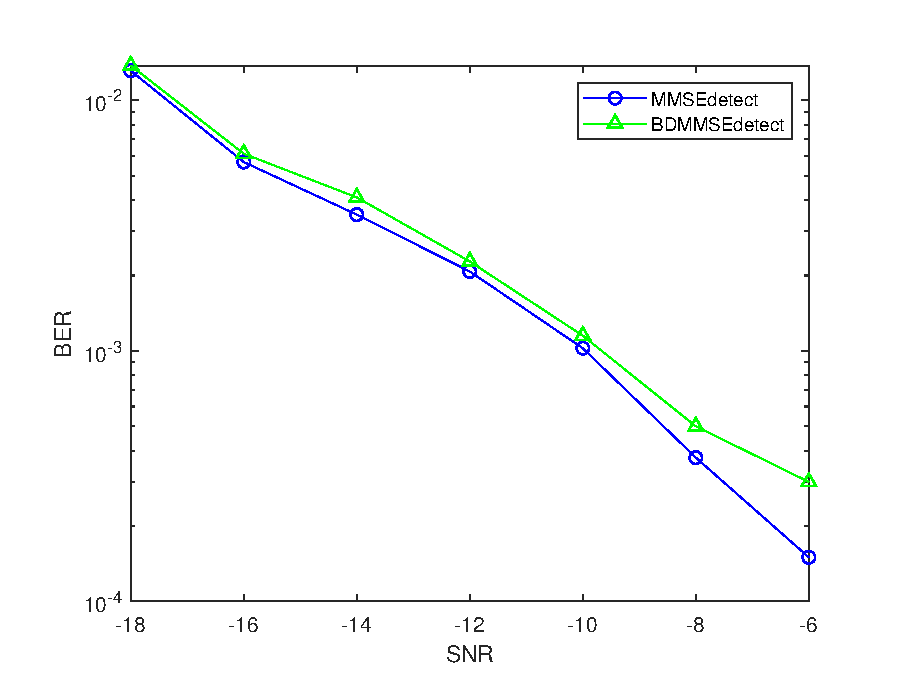
\includegraphics[width=0.55\textwidth]{img/3_5.eps} \caption{4用户2天线单流普通MMSE与波束域MMSE对比}
\end{figure}
\begin{figure}[htbp!]
	\centering 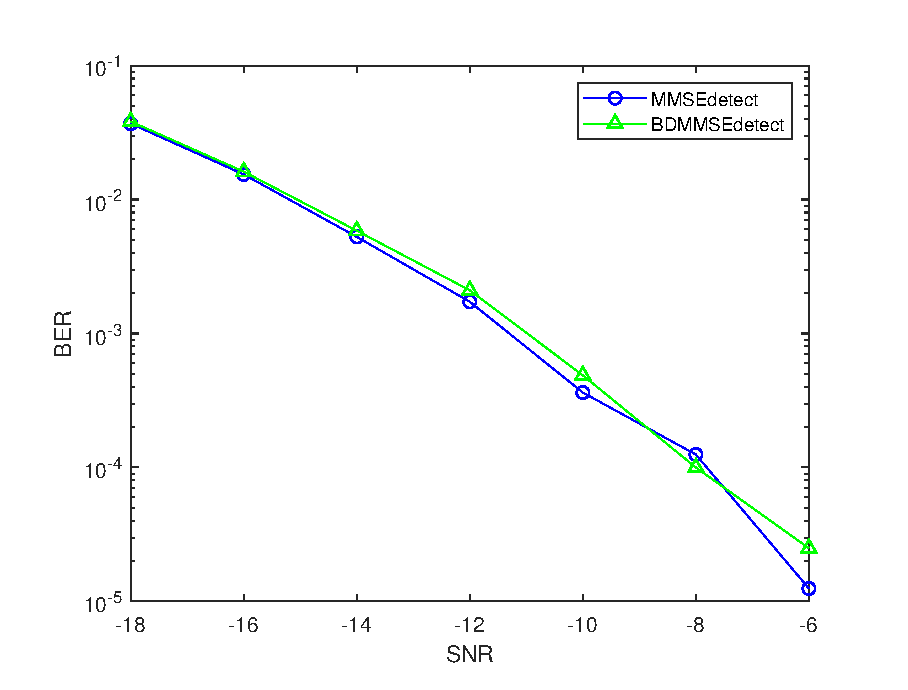
\includegraphics[width=0.55\textwidth]{img/3_6.eps} \caption{4用户2天线多流普通MMSE与波束域MMSE对比}
\end{figure}
\begin{figure}[htbp!]
	\centering 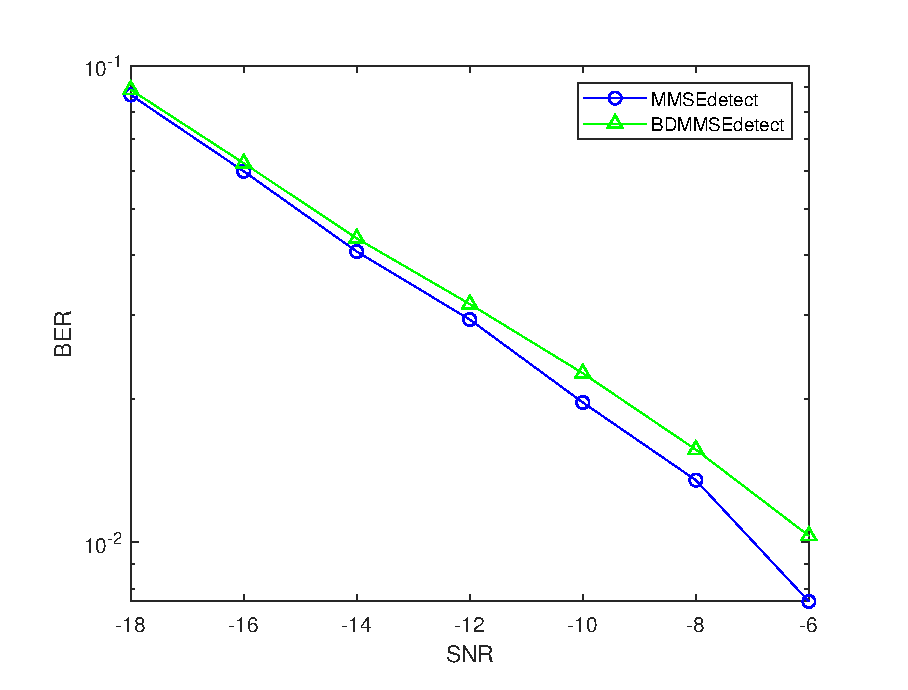
\includegraphics[width=0.55\textwidth]{img/3_7.eps} \caption{4用户4天线多流普通MMSE与波束域MMSE对比}
\end{figure}

\begin{table}[htbp]
	\centering
	\caption{\label{tab:complexity}MMSE复杂度分析表}
	\begin{tabular}{ll}
		\toprule
		方法 & 复杂度 \\
		\bottomrule
		普通MMSE & $O(N_R^3)$ \\
		QR分解(Givens 或 Householder 变换)MMSE & $\Theta(N_R^2)$ \\
		QR分集波束域MMSE & $O((N_uN_{beam})^2)$ \\
	    \bottomrule
	\end{tabular}
\end{table}


\section{本章小结}
本章主要研究基于MMSE检测的低复杂度算法,并分析其与普通MMSE检测的检测性能对比,是否能在降低计算复杂度的同时保持检测性能。本章首先介绍本文所需要使用的系统模型,以及本章节需要用到的波束域理论以及下章节可能用的统计信道的符号表达。并且将本章具体叙述的系统模型作为每个检测算法的系统模型。然后本文推导了MMSE检测估计的原理以及MMSE的仿真结果并将其作为测试低复杂度算法是否保证检测性能的基准。接着本文根据MMSE算式特点,利用QR分解进行数学层面上的化简推导,得到了复杂度稍低的QR分解的MMSE算法,因为其是严格数学推导的,所以QR分解的MMSE算法的性能相较普通MMSE接收机并没有区别。然后利用QR分解中Givens变换方法以及Householder变换方法在矩阵稀疏情况下复杂度会降低,从而可以利用波束域信道稀疏特性进行进一步的复杂度化简。而本文推导严格稀疏的矩阵需要基站侧天线数无穷大,所以利用数学公式无法得到严格系数的波束域矩阵,这里本文做了近似处理,并利用近似结果进行测试,仿真结果显示低复杂度的MMSE接收机在降低复杂的同时能够很好保证性能。


\chapter{基于多项式展开接收机及复杂度优化}
\section{引言}
基于MMSE检测准则,利用检测矩阵约等式,利用系数代替检测矩阵,衍生出了PE接收机,即多项式展开(polynomial expansion)接收机。PE接收机其一定程度降低了复杂度,但是其不能很好的解决当上行信道用户天线总数比较大时系统检测矩阵系数计算仍然很复杂的问题。所以,本章节还会提出一种基于算子自由度的算法,将多项式展开得到的系数替换为确定性等同。通过替换可以略过计算多项式展开的计算,同时降低PE接收机的复杂度。本章将推导利用算子自由度理论证明算子自由等同能够代替系数,在PE接收机的基础上进一步的降低大规模MIMO的计算复杂度,并且涉及到的小规模的矩阵求逆和递推系数计算将更容易应用到硬件上,从提高其检测时延。
\section{PE接收机原理及仿真}
通过上述计算过程,可以知道在用户数较多用户天线数较多的情况下,MMSE接收机的复杂度将会非常的高\cite{LuAnAn}。所以基于MMSE接收机的基本原理有提出了多项式展开的方法对MMSE矩阵进行合理的化简,化简表达式如下
\begin{gather}\label{key}
\mathbf{W} = (\mathbf{H}\mathbf{H}^H + \sigma^2 \mathbf{I})^{-1}\mathbf{H}^H  \nonumber \\
\mathbf{x}_{MMSE} = \mathbf{W} \mathbf{y}  
\end{gather}
利用Cayley hamilton理论,$(\mathbf{H}^H\mathbf{H}+\sigma_z^2\mathbf{I})^-1$可以表达为
\begin{equation}\label{key}
(\mathbf{H}^H\mathbf{H}+\sigma^2_z\mathbf{I})^{-1} = \sum_{i=1}^M c_i(\mathbf{H}^H \mathbf{H}+\sigma^2_z\mathbf{I})^i
\end{equation}
而等式根据多项式分解可以写为下式
\begin{equation}\label{key}
\sum_{i=1}^M c_i(\mathbf{H}^H \mathbf{H}+\sigma^2_z\mathbf{I})^i=\sum_{i=1}^M b_i(\mathbf{H}^H\mathbf{H})^i
\end{equation}
PE接收机可以通过约等式降低复杂度
\begin{equation}\label{key}
(\mathbf{H}^H\mathbf{H}+\sigma^2\mathbf{I})^{-1} \approx \sum_{i=1}^{L} b_{PE,i}^{(L)}(\mathbf{H}^H\mathbf{H})^{i-1}
\end{equation}
仍然利用MMSE接收机的判断准则来计算多项式系数
\begin{equation}\label{key}
\mathrm{arg} \min_{b_{PE}^{(L)}} \mathbb{E}_x \left\lbrace \| \mathbf{x}-\sum_{i=1}^{L}b_{PE,i}^{(L)}(\mathbf{H}^H\mathbf{H})^{i-1}\mathbf{H}^Hy \| \right\rbrace
\end{equation}
并令$\mathbf{b}^{(L)}_{PE}$ 表示 $b_{PE,i}^{(L)}$的合集。这里考虑的$L \leq M$,$M$为发送端用户天线总数
令
\begin{gather}\label{key}
\mathbf{B}_N = \mathbf{H}\mathbf{H}^H \nonumber \\
\mu_k = \frac{1}{N} \mathrm{tr}(\mathbf{B}_N^k) \nonumber
\end{gather}
其中$\frac{1}{N} \mathrm{tr}(\mathbf{B}_N^k)$指的是信道的经验矩。
\begin{gather}\label{key}
[\mathbf{\Phi}_{PE}]_{ij} = \mu_{i+j} + \sigma_{z}^2 \mu_{i+j-1} \nonumber \\
\left[\mathbf{\alpha}_{PE}\right]_i = \mu_i
\end{gather}

通过上式可以得到PE接收机检测表达式
\begin{equation}\label{key}
\hat{x}_{PE}^{(L)} = \sum_{i=1}^{L}b_{PE,i}^{(L)}(\mathbf{H}^H\mathbf{H})^{i-1}  \mathbf{H}^H y
\end{equation}
利用上章系统模型
\begin{equation}\label{key}
	\mathbf{y} = \sum_{i=1}^{K} \mathbf{H}_i \mathbf{x}_i + \mathbf{Z}
\end{equation}
与MMSE类似的,$\mathbf{H}$代表$[\mathbf{H}_1,\mathbf{H}_2,...,\mathbf{H}_K]$,令$\mathbf{x}$代表$[\mathbf{x}_1^T,\mathbf{x}_2^T,...,\mathbf{x}_K^T]$,带入上面的判断准则。

而上文也提到了MMSE的复杂度主要来自于矩阵求逆的计算,上部分提出利用QR分解的形式进行化简矩阵求逆的公式,而这部分主要使用的是Cayley hamilton理论将矩阵求逆转换为多项式分解,再利用约等式对多项式分解的项数进行减少,从而降低计算复杂度。PE接收机的复杂度一定程度上取决PE接收机的阶数,而根据$\sum_{i=1}^{L} b_{PE,i}^{(L)}(\mathbf{H}^H\mathbf{H})^{i-1}$又被称为Krylov 域的计算,其计算复杂度为$O(M^2)$,而计算系数的需要的复杂度为$O(L*M^2)$,L为阶数。L相对于M小很多,而这两部分是相加关系,所以此时的复杂度比原始MMSE要小很多,而其并不会依赖于矩阵是否稀疏。

考虑的为BPSK调制,分别考虑用户单天线和用户多天线,多天线时设置为2和4,判决采用硬判决判决采用硬判决。多天线单流的多天线结果利用平均值进行判断。
\begin{table}[htbp]
	\centering
	\caption{\label{tab:test}PE接收机仿真参数设置}
	\begin{tabular}{ll}
		\toprule
		参数 &  设置值 \\
		\bottomrule
		场景 &  郊区宏蜂窝 \\
		\bottomrule
		基站侧天线数 & 128 \\
		\bottomrule
		用户数天线	& 1 \quad or\quad2 or\quad4\\
		\bottomrule
		用户数	& 4 \\
		\bottomrule
		天线间距 & 0.5$\lambda$ \\
		\bottomrule
		路径数 & 6 \\
		\bottomrule
		用户采样数量 & 10000 \\
		\bottomrule
	\end{tabular}
\end{table}


从图4.1,4.2,4.3来看,在用户天线数为2,用户数为4时,PE接收机在阶数为3的情况下PE接收机能够逼近MMSE接收机的性能,而从图4.4来看在面对用户发送天线数量更多的情况,需要阶数更高的PE接收机。
可以发现PE接收机在阶数比较小的情况下,仍然可以很好的处理不同用户之间带来的干扰。当然从波束域信道上,如果可以很好的分配用户的波束域资源的话,那么针对用户间干扰的所需要的PE接收机的阶数将会进一步的降低,相对应的该系统的带宽可能会收到影响。当用户多天线单流的情况下,PE接收机的性能更加接近MMSE接收机。从图4.4来看PE接收机在处理用户多天线多流的情况,根据用户天线数还是有一些区别,随着用户天线数的增多,用户天线之间的互相干扰同样会增大,实际情况中特别是当用户数天线大于2,用户天线数间隔会超出波长时,处于波长整数倍情况下会接受到更多来自另外天线的干扰。从仿真结果来看,当双天线时,阶数为3的PE的接收机尚能逼近MMSE性能,而在用户四天线的情况下,阶数为3的PE接收机已经和MMSE的结果产生了差距,需要更高的阶数来应对用户多天线的情况。PE接收机在降低复杂度情况下能保持很好的接收检测性能。

\begin{figure}[htbp!]
	\centering 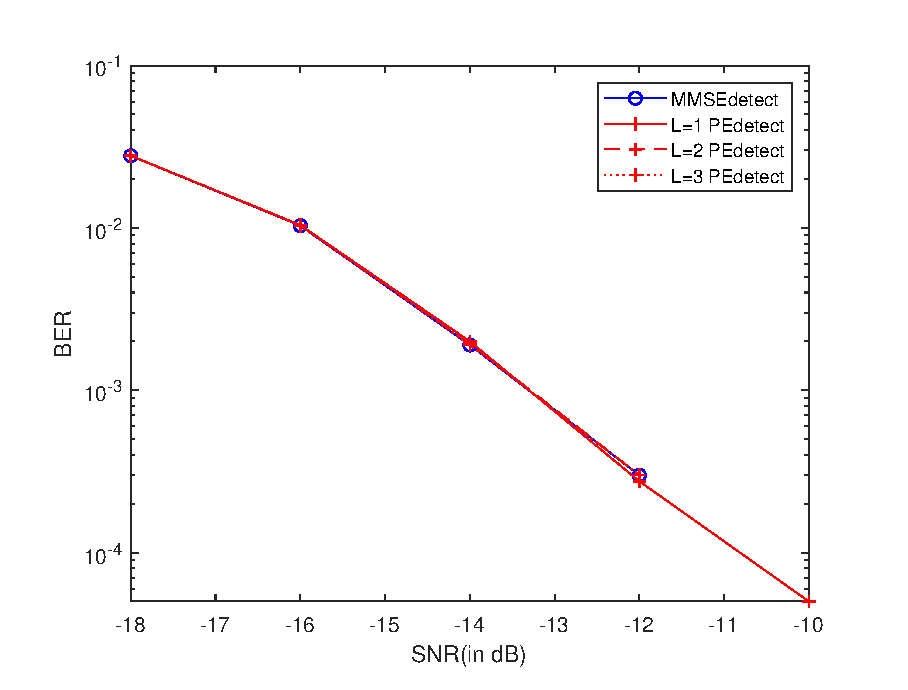
\includegraphics[width=0.55\textwidth]{img/4_1.eps} \caption{4用户单天线PE接收机与MMSE接收机比较}
\end{figure}
\begin{figure}[htbp!]
	\centering 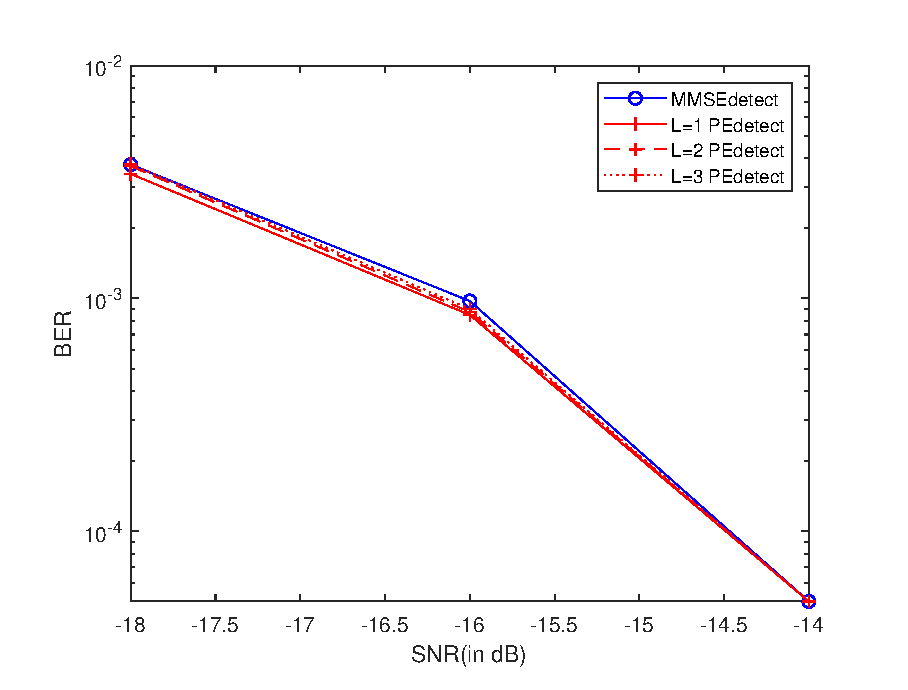
\includegraphics[width=0.55\textwidth]{img/4_2.eps} \caption{4用户2天线单流PE接收机与MMSE接收机比较}
\end{figure}
\begin{figure}[htbp!]
	\centering 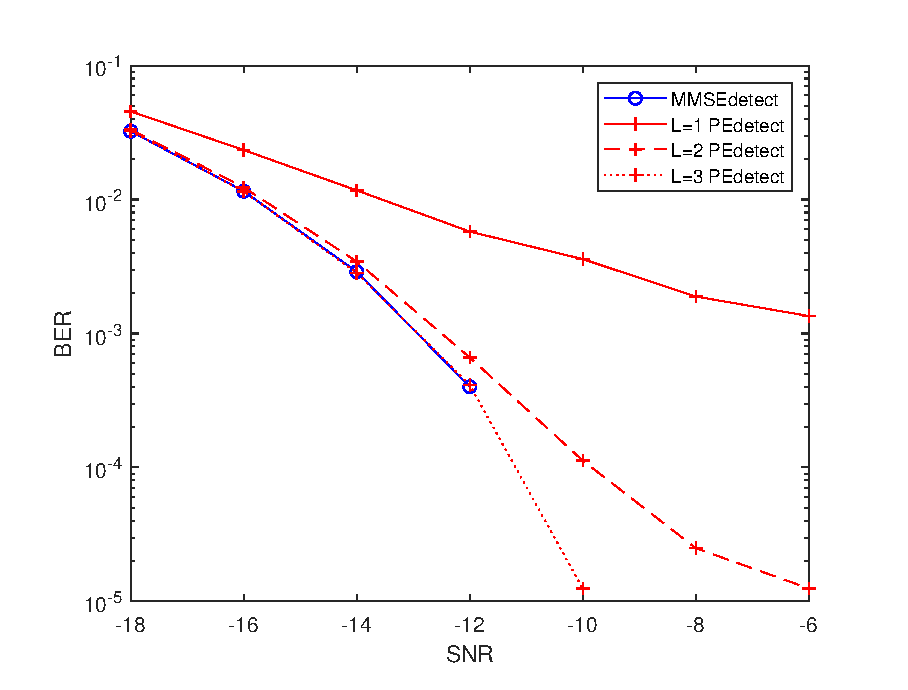
\includegraphics[width=0.55\textwidth]{img/4_3.eps} \caption{4用户2天线多流PE接收机与MMSE接收机比较}
\end{figure}
\begin{figure}[htbp!]
	\centering 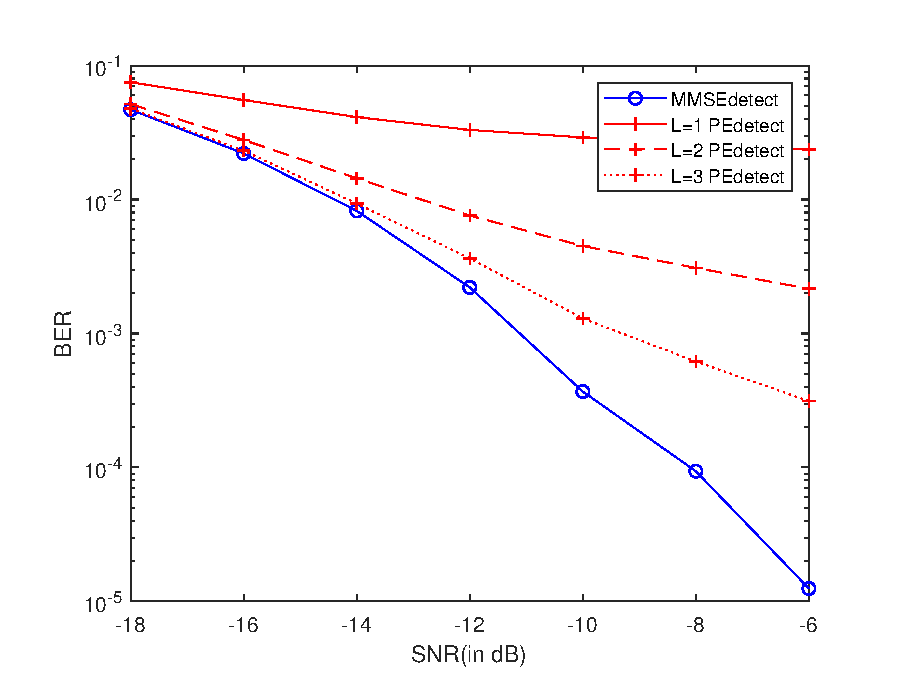
\includegraphics[width=0.55\textwidth]{img/4_4.eps} \caption{4用户4天线多流PE接收机与MMSE接收机比较}
\end{figure}
\section{算子自由度原理}
上面为使用MMSE准则的多项式接收机,可以注意到当信道矩阵的维度较大的时候,利用经验矩计算每个信道同样会有较大的复杂度。但是在信道慢变的情况下,数据CSI变化得非常的慢,可以利用确定性等同$\overline{\mu}_k$代替$\mu_k$,进一步降低复杂度。此时,PE接收机只用计算$\sum_{i=1}^{L} b_{PE,i}^{(L)}(\mathbf{H}^H\mathbf{H})^{i-1}$ 即可。计算复杂度只有$O(M^2)$。这里提出了利用算子自由度从而得到$\overline{\mu}_k$的方法。考虑本文是建立在大规模MIMO背景下的,所以本章开头提到的基站侧接收天线数量$N_R$可以看作是数量相当大。

当$N \rightarrow \infty$,有$\mu - \mathbb{E}[\mu] \rightarrow 0$。即
\begin{equation}\label{key}
\lim_{N \rightarrow \infty} \mathbb{E}[\mu_k] -\mu_k =0
\end{equation}
不过即使这步趋近并不能很好的获得,仍然可以利用下面的公式进行替代原来的方法。
\begin{gather}\label{key}
[\mathbf{\Phi}_{PE}]_{ij} = \mathbb{E}[\mu_{i+j}] + \sigma_{z}^2 \mathbb{E}[\mu_{i+j-1}] \nonumber \\
\left[\mathbf{\alpha}_{PE}\right]_i = \mathbb{E}[\mu_i]
\end{gather}
但是式(3.41)的请况并不在本文的考虑范围内,所以接下来本文将用$\mathbb{E}[\mu]$代替$\mu$。而本文提出的利用算子自由度,即将期望$\mathbb{E}[\mu]$由数转为算子,利用算子自由度对其进行计算。
这里本文简要介绍算子自由度的定义。

线性映射$E$是一个条件期望,如果其满足对于所有$b$,都有$E[b]=b$,对于所有$x$属于集合$\mathcal{A}$,$b_1,b_2$属于集合$\mathcal{B}$都有$E[b_1\mathcal{X}b_2]= b_1E[\mathcal{X}]b_2$。令$\mathcal{A}$表示酉代数,$\mathcal{B}$表示酉子代数,$E:\mathcal{A}->\mathcal{B}$是一个条件期望。则称$(\mathcal{A},E)$是$\mathcal{B}$算子值的自由空间。$\mathcal{B}$算子值概率空间元素成为$\mathcal{B}$算子值随机变量。$\mathcal{B}$算子值自由度乘法映射$\lbrace f_{\pi} \rbrace _{\pi \in NC(n)}:\mathcal{A}^n \rightarrow \mathcal{B}$
\begin{equation}\label{key}
f_{\pi_1 \bigsqcup \pi_2}^{\mathcal{B}}(\mathcal{X}_1,\mathcal{X}_2,...,\mathcal{X}_n) = f_{\pi_1}^{\mathcal{B}}(\mathcal{X}_1,\mathcal{X}_2,...,\mathcal{X}_n)f_{\pi_2}^{\mathcal{B}}(\mathcal{X}_1,\mathcal{X}_2,...,\mathcal{X}_n)
\end{equation}
$NC(n)$只n长度中不互相交叉的段,$\pi_1$和$\pi_2$就是其中的两个。

用$\mathcal{V}_{\pi}^{\mathcal{B}}(\mathcal{X}_1,\mathcal{X}_2,...,\mathcal{X}_n) = E((\mathcal{X}_1\mathcal{X}_2...\mathcal{X}_n))$定义$\mathcal{B}$算子值自由度乘法映射$\mathcal{V}_{\pi}^{\mathcal{B}} :\mathcal{A}^n \rightarrow \mathcal{B}$
。而算子的累差值同样也是算子自由度乘法映射可以由下式定义
\begin{equation}\label{key}
E((\mathcal{X}_1\mathcal{X}_2...\mathcal{X}_n)) = \sum_{\pi \in NC(n)} \mathcal{K}_{\pi}^{\mathcal{B}}(\mathcal{X}_1,\mathcal{X}_2,...,\mathcal{X}_n)
\end{equation}
则有
\begin{equation}\label{key}
\sum_{\pi \in NC(n)} \mathcal{K}_{\pi}^{\mathcal{B}}(\mathcal{X}_1,\mathcal{X}_2,...,\mathcal{X}_n) = \mathcal{V}_{\sigma}^{\mathcal{B}}(\mathcal{X}_1,\mathcal{X}_2,...,\mathcal{X}_n)\mu(\sigma,\pi)
\end{equation}
利用M\"{o}bius函数可以写为
\begin{equation}\label{key}
\mathcal{K}_{\pi}^{\mathcal{B}}(\mathcal{X}_1,\mathcal{X}_2,...,\mathcal{X}_n) = \sum_{\sigma<\pi, \in \pi \in NC(n)} \mathcal{V}_{\sigma}^{\mathcal{B}}(\mathcal{X}_1,\mathcal{X}_2,...,\mathcal{X}_n)\mu(\sigma,\pi)
\end{equation}
随机变量$\mathcal{X}$的$\mathcal{B}$算子R阶变换为
\begin{equation}\label{key}
\mathcal{R}_{\mathcal{X}}(b)=\sum_{n \geq 0} \mathcal{K}_{n+1}^{\mathcal{B}}(\mathcal{X}b,\mathcal{X}b,...,\mathcal{X}b,\mathcal{X}b,\mathcal{X})
\end{equation}
如有一个$\mathcal{B}$算子随机变量$\mathcal{X} \in \mathcal{A}$有
\begin{equation}\label{key}
\mathcal{R}_{\mathcal{X}}(b)=\mathcal{K}_2(\mathcal{X}b,\mathcal{X})
\end{equation}
则称其为$\mathcal{B}$算子半圆变量。

下文将主要介绍如何利用上面的公式得到$\overline{\mu}$的等同确定量。根据(3.13)(3.14)可以得到$\mathbf{H} = \overline{\mathbf{H}} + \tilde{\mathbf{H}}$
令
\begin{equation}\label{key}
\overline{\mathbf{X}} = \left(
\begin{array}{cc}
0_N & \overline{\mathbf{H}} \\
\overline{\mathbf{H}}^H & 0_M
\end{array}
\right)
\end{equation}
与
\begin{equation}\label{key}
\tilde{\mathbf{X}} = \left(
\begin{array}{cc}
0_N & \tilde{\mathbf{H}} \\
\tilde{\mathbf{H}}^H & 0_M
\end{array}
\right)
\end{equation}
并令$\mathbf{X} = \tilde{\mathbf{X}} + \overline{\mathbf{X}}$,$\tilde{\mathbf{W}}_k$代表$\mathbf{M}_k \odot \mathbf{W}_k$,$\eta(\mathbf{D})$代表$\mathbb{E}\lbrace \tilde{\mathbf{X}} \mathbf{D} \tilde{\mathbf{X}} \rbrace $ 。 根据信道模型,可以得到$\mathbb{E}[\mu_k]$与$\mathbf{X}$的矩有关。
又有
\begin{equation}\label{key}
\mathbf{X}^2 = \left(
\begin{array}{cc}
\mathbf{H}\mathbf{H}^H & 0_{N*M} \\
0_{M*N} & \mathbf{H}^H\mathbf{H}
\end{array}
\right)
\end{equation}
又令
\begin{equation}\label{key}
\tilde{\mathbf{X}}_k = 
\left(
\begin{array}{cc}
0_N & \hat{\mathbf{H}}_k \\
\hat{\mathbf{H}}^H_k & 0_M
\end{array}
\right)
\end{equation}
其中$\hat{\mathbf{H}}_k$代表$[ 0_{N*M_1} \ldots \tilde{\mathbf{H}}_k \quad 0_{N*M_{k+1}} \ldots]$,所以有下式
\begin{equation}\label{key}
\tilde{\mathbf{X}} = \sum_{k=1}^{K} \tilde{\mathbf{X}}_k
\end{equation}
根据上面信道模型,可以写出$\tilde{\mathbf{H}}_k = \mathbf{U}_k \tilde{\mathbf{W}}_k \mathbf{V}_k^H$,同时可以改写$\tilde{\mathbf{X}}$
\begin{equation}\label{key}
\tilde{\mathbf{X}}_k = \mathbf{A}_k \hat{\mathbf{W}} \mathbf{A}^H
\end{equation}
其中$\hat{\mathbf{W}}$可以用下式表示
\begin{equation}\label{key}
\left(
\begin{array}{ccccc}
0_N & \ldots & \tilde{\mathbf{W}} & 0_{N*M_{k+1}} & \ldots \\
\vdots & \ddots & \ldots & \ldots & \ldots \\
\tilde{\mathbf{W}}^H & \ldots & 0_{M_k * M_k} & 0_{M_k*M_{k+1}} & \ldots \\
0_{M_{k+1}*N} & \ldots & 0_{M_{k+1} *M_k} & 0_{M_{k+1}*M_{k+1}} & \ldots \\
\vdots & \ldots & \vdots & \vdots & \ddots
\end{array}
\right)
\end{equation}
\begin{equation}\label{key}
\mathbf{A}_k = \mathrm{diag}(\mathbf{U}_k,0_{M_1},\ldots,\mathbf{V}_k,0_{M_{k+1}},\ldots)
\end{equation}

通过替换$\hat{\mathbf{W}}$中的独立高斯变变量为相同方差的自由圆形变量,可以获得自由确定性等同$\hat{\mathcal{W}}$。而此时,令$\hat{\mathcal{X}}_k = \mathbf{A}_k \hat{\mathcal{W}}_k \mathbf{A}_k$ 则也可以用自由确定性等同$\mathcal{X}$代替$\mathbf{X}$。一般的,自由确定性等同$\mathcal{X}$和原始模型数据$\mathbf{X}$在L趋近于无穷时都有相同算子分布。令$\mathcal{B}_N$代表$<\mathcal{X}>_N$。$<\mathcal{X}>_N$指的是$\mathcal{X}$行列下标1到N的子矩阵。
令$F_{\mathbf{B}_N}(\lambda)$代表随机矩阵$\mathbf{B}_N$的元素的累计分布。令$\mathbb{C}^+$代表集合$\lbrace z\in \mathbb{C}: \mathcal{J}(z) > 0 \rbrace$。参考文献,$z \in \mathbb{C}^+$的柯西变换$G_{\mathbf{B}_N}(z)$
\begin{equation}\label{key}
G_{\mathbf{B}_N}(z) = \int_0^\infty \frac{1}{z-\lambda} dF_{\mathbf{B}_N}(\lambda) = \frac{1}{N} \mathbb{E}\lbrace \mathrm{tr}(z \mathbf{I}_N - \mathbf{B}_N)^{-1}\rbrace
\end{equation}
对于所有代表柯西变换的$F_{\mathbf{B}_N}$,都有反变换,可以写成下面形式
\begin{equation}\label{key}
F_{\mathbf{B}_N}(\lambda) = -\frac{1}{\pi} \lim_{\epsilon \rightarrow 0^+} \int_{-\infty}^{\lambda}  \mathcal{J}(\mathbf{G}_{\mathbf{B}_N}(x+i\epsilon))dx
\end{equation}
参考文献,有柯西变换$G_{\mathcal{B}_N}(z)$是$G_{\mathbf{B}_N}(z)$的确定性等同
\begin{equation}\label{key}
\lim_{N \rightarrow \infty}(G_{\mathbf{B}_N}(z)-G_{\mathcal{B}_N}(z)) = 0
\end{equation}
$\mathcal{B}_N$是$\mathbf{B}_N$的确定性等同。并且有这样$\overline{\mu}_k = \frac{1}{N}\mathbb{E}[\mathrm{tr}(\mathcal{B}_N^k)]$。并且可作出这样的近似
\begin{equation}\label{key}
\lim_{N \rightarrow \infty} \mathbb{E}[\mu_k] -\overline{\mu_k} =0
\end{equation}
参考文献\cite{lu2015low},给出的$E\lbrace\mu_m\rbrace$和$\mu_m$做比较,参见表\ref{tab:Emu1}\ref{tab:Emu2}\ref{tab:Emu3}

%\begin{figure}[htbp!]
	%\centering 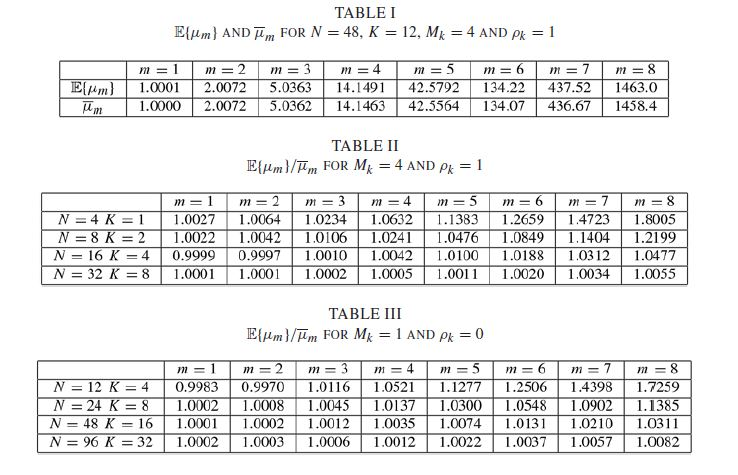
\includegraphics[width=1\textwidth]{img/3_6.jpg} 
%\end{figure}
\begin{table}[htbp]
	\centering
	\caption{\label{tab:Emu1} $E\lbrace\mu_m\rbrace$和$\mu_m$ 条件 :$N_R =48,K=12,M_k=4$}
	\begin{tabular}{|c|c|c|c|c|c|c|c|c|}
		\hline
		\quad &  m=1 &  m=2 &  m=3 &  m=4 &  m=5 &  m=6 &  m=7 &  m=8  \\
		\hline
		$E\lbrace\mu_m\rbrace$ &  1.0001 & 2.0072 & 5.0363 & 14.1491 & 45.5792 &134.22 &437.52 &1463.0 \\
		\hline
		$\mu_m$ &  1.0001 & 2.0072 & 5.0362 & 14.1463 & 45.5764 &134.07 &436.67 &1458.4 \\
		\hline
	\end{tabular}
\end{table}

\begin{table}[htbp]
	\centering
	\caption{\label{tab:Emu2} $E\lbrace\mu_m\rbrace$/$\mu_m$ 条件: $M_k=1$}
	\begin{tabular}{|c|c|c|c|c|c|c|c|c|}
		\hline
		\quad &  m=1 &  m=2 &  m=3 &  m=4 &  m=5 &  m=6 &  m=7 &  m=8  \\
		\hline
		$N=12,K=f$ &  0.9983 & 0.9970 & 1.0234 & 1.0521 & 1.2583 & 1.2657 & 1.4723 &1.8005 \\
		\hline
		$N=24,K=8$ &  1.0002 & 1.0008 & 1.0045 & 1.0241 & 1.0476 & 1.0549 & 1.1404 &1.2199 \\
		\hline
		$N=48,K=16$ &  1.0001 & 1.0002 & 1.0012 & 1.0035 & 1.0100 & 1.0138 & 1.0312 &1.0427 \\
		\hline
		$N=96,K=32$ &  1.0002 & 1.0001 & 1.0002 & 1.0012 & 1.0011 & 1.0022 & 1.0034 &1.0055 \\
		\hline
	\end{tabular}
\end{table}

\begin{table}[htbp]
	\centering
	\caption{\label{tab:Emu3} $E\lbrace\mu_m\rbrace$/$\mu_m$ 条件: $M_k=4$}
	\begin{tabular}{|c|c|c|c|c|c|c|c|c|}
		\hline
		\quad &  m=1 &  m=2 &  m=3 &  m=4 &  m=5 &  m=6 &  m=7 &  m=8  \\
		\hline
		$N=4,K=1$ &  1.0027 & 0.9977 & 1.0116 & 1.0521 & 1.1227 & 1.2659 & 1.4727 &1.7259 \\
		\hline
		$N=8,K=2$ &  1.0022 & 1.0009 & 1.0045 & 1.0137 & 1.00476 & 1.0849 & 1.1404 &1.1138 \\
		\hline
		$N=16,K=4$ &  0.9999 & 1.0007 & 1.0012 & 1.0035 & 1.0100 & 1.0188 & 1.0012 &1.0311 \\
		\hline
		$N=32,K=8$ &  1.0001 & 1.0001 & 1.0006 & 1.0012 & 1.0011 & 1.0020 & 1.0034 &1.0082 \\
		\hline
	\end{tabular}
\end{table}

将原始模型的矩阵矩的确定性等同转换到算子自由度模型上。接着可以利用上文提到的算子自由度的定理和公式来计算$\overline{\mu}_k$。下文简要介绍计算理论,令$\mathcal{B}$表示代数$\mathcal{M}_{N+M}(\mathbb{C})$。利用元素的累差可以就计算出$\tilde{\mathcal{X}}_1,\tilde{\mathcal{X}}_2,\ldots,\tilde{\mathcal{X}}_K$。通过计算,可以得到所有的$\mathcal{B}$累差各不相同,并且只有第二阶$\mathcal{B}$算子累差是非零矩阵。因此$\tilde{\mathcal{X}}_1,\tilde{\mathcal{X}}_2,\ldots,\tilde{\mathcal{X}}_K$关于$\mathcal{B}$自由,并且每一个$\tilde{\mathcal{X}}$都是关于$\mathcal{B}$的半圆形变量。并且非零的累差可以用下式表示
\begin{equation}\label{key}
\mathcal{K}_2(\tilde{\mathcal{X}},\mathbf{D}\tilde{\mathcal{X}})=\mathbb{E}[\mathcal{X}\mathbf{D}\tilde{\mathcal{X}}]
\end{equation}
又因为上文所做的自由确定等同与原始模型的对应,还可以得到下式
\begin{equation}\label{key}
\mathbb{E}[\mathcal{X}\mathbf{D}\tilde{\mathcal{X}}]=
\mathbb{E}[\mathbf{X}\mathbf{D}\tilde{\mathbf{X}}] = \eta(\mathbf{D})
\end{equation}
同时,所有的高阶$\mathcal{B}$算子累差都是零矩阵。所以有下式表示一阶$\mathcal{B}$算子累差
\begin{equation}\label{key}
\mathcal{K}_2(\overline{\mathbf{X}}) = \overline{\mathbf{X}}
\end{equation}
之前有$\mathcal{X}=\overline{\mathbf{X}}+\tilde{\mathcal{X}}$因为$\overline{\mathbf{X}}\in \mathcal{B}$,本文$\overline{\mathbf{X}}$和$\overline{\mathcal{X}}$关于$\mathcal{B}$算子自由。
则有
\begin{gather}\label{key}
\mathcal{K}_1(\mathcal{X}) = \mathcal{K}_1(\overline{\mathbf{X}}) + \mathcal{K}_1(\overline{\mathcal{X}}) = \overline{\mathbf{X}} \nonumber\\
\mathcal{K}_2({\mathcal{X}},\mathbf{D}{\mathcal{X}})=\mathcal{K}_2(\tilde{\mathcal{X}},\mathbf{D}\tilde{\mathcal{X}}) + \mathcal{K}_2(\overline{\mathcal{X}},\mathbf{D}\overline{\mathcal{X}})\\ =\mathbb{E}[\mathcal{X}\mathbf{D}\tilde{\mathcal{X}}]\nonumber = 
\mathbb{E}[\mathbf{X}\mathbf{D}\tilde{\mathbf{X}}] = \eta(\mathbf{D})
\end{gather}
由此本文得到下面的推论来计算$\mathbb{E}[\mathcal{X}^k]$从而能够推导到$\overline{\mu}_k$。下面的递推公式可以计算出$\mathbb{E}[\mathcal{X}^k]$。
\begin{eqnarray}\label{key}
\mathbb{E}[\mathcal{X}^{2m+2}]=\overline{\mathbf{X}}\mathbb{E}[\mathcal{X}^{2m+1}]+\sum_{j=0}^{m}\eta(\mathbb{E}[\mathcal{X}^{2j}])\mathbb{E}[\mathcal{X}^{2m-2j}]  \\
\mathbb{E}[\mathcal{X}^{2m+1}]=\overline{\mathbf{X}}\mathbb{E}[\mathcal{X}^{2m}]+\sum_{j=0}^{m}\eta(\mathbb{E}[\mathcal{X}^{2j}])\mathbb{E}[\mathcal{X}^{2m-2j-1}] 
\end{eqnarray}
其中m是自然数,$\mathbb{E}[\mathcal{X}^0] = \mathbf{I}_n$

用代数形式表示$\mathcal{D}$
\begin{equation}\label{key}
\mathcal{D} = \mathrm{diag}(\mathcal{M}_N(\mathbb{C}),\mathcal{M}_{M_1}(\mathbb{C}),...,\mathcal{M}_{M_K}(\mathbb{C}))
\end{equation}
本文在论文模型部分讨论过所选用统计模型
\begin{equation}\label{key}
\mathbf{H} = \mathbf{U}_{r}\tilde{\mathbf{H}}\mathbf{U}_{t}^{H} = \mathbf{U}_{r}(\mathbf{D}+\mathbf{M}\odot \mathbf{H}_{idd})\mathbf{U}_{t}^{H}
\end{equation}
考虑其中的$\mathbf{D}$为0,在此算子自由度模型中即$\overline{\mathbf{X}} = 0_N$。则可以得到下面的递推公式。
\begin{gather}\label{key}
\mathbb{E}[\mathcal{B}^{m+1}_N] = \sum_{j=0}^{m}(\sum_{k=0}^{K}\tilde{\eta_k}(\mathbf{S}_{jk}))\mathbb{E}[\mathcal{B}_N^{m-j}] \\
\mathbf{S}_{(m+1)k} =\sum_{j=0}^{m}\eta(\mathbb{E}(\mathcal{B}_N^j))\mathbf{S}_{m-j}k
\end{gather}
其中m是自然数,$\mathbb{E}[\mathcal{B}_N^0]=\mathbf{I}_N$和$\mathbf{S}_{0k}=\mathbf{I}_{M_k}$。
利用此递推公式,可以进一步进行低复杂度PE接收机的推导。

\section{低复杂度的PE接收机}
以上是基于算子自由度理论,下面将叙述低复杂多项式展开(PE)接收机的算法。如上文所叙述的,本文考虑的是$\overline{\mathbf{X}} = 0_N$的情况,所以低复杂度PE接收机首先根据递推公式
\begin{gather}\label{key}
\mathbb{E}[\mathcal{B}^{m+1}_N] = \sum_{j=0}^{m}(\sum_{k=0}^{K}\tilde{\eta_k}(\mathbf{S}_{jk}))\mathbb{E}[\mathcal{B}_N^{m-j}] \\
\mathbf{S}_{(m+1)k} =\sum_{j=0}^{m}\eta(\mathbb{E}(\mathcal{B}_N^j))\mathbf{S}_{m-j}k
\end{gather}
计算$\mathbb{E}[\mathcal{B}_N^{m}]$和$\mathbf{S}_{(m)k}$。
\begin{equation}\label{key}
\overline{\mu}_{m} = \frac{1}{N} \mathrm{tr}(\mathbb{E}[\mathcal{B}_N^{m}])
\end{equation}
令维度为$L*L$的矩阵$\overline{\Phi}_{PE}$为
\begin{equation}\label{key}
[\overline{\Phi}_{PE}]_{ij} = \overline{\mu}_{i+j} + \sigma_z^2 \overline{\mu}_{i+j-1}
\end{equation}
令向量$\bm{\alpha}_{PE}$为
\begin{equation}\label{key}
[\overline{\bm{\alpha}}_{PE}]_i = \overline{\mu}_i
\end{equation}
利用上面两等式计算出估计系数为
\begin{equation}\label{key}
\overline{\mathbf{b}}_{PE}^{L} = \overline{\Phi}_{PE}^{-1} [\overline{\bm{\alpha}}_{PE}]
\end{equation}
带入系数PE接收机判决公式
\begin{equation}\label{key}
\hat{x}_{LPE}^{(L)} = \sum_{i=1}^{L}\overline{b}_{PE,i}^{(L)}(\mathbf{H}^H\mathbf{H})^{i-1}  \mathbf{H}^H y
\end{equation}

上面描述低复杂度PE接收机利用确定性等同进行计算,因为省略了计算多项式展开的系数的过程,那么用确定量计算的PE接收机计算复杂度将仅仅是Krylov域的计算,其计算复杂度为$O(M^2)$,M为接收天线总数。
考虑的为BPSK调制,分别考虑用户单天线和用户多天线,多天线时设置为2和4,判决采用硬判决判决采用硬判决。多天线单流的多天线结果利用平均值进行判断。
\begin{table}[htbp]
	\centering
	\caption{\label{tab:test}LPE接收机仿真参数设置}
	\begin{tabular}{ll}
		\toprule
		参数 &  设置值 \\
		\bottomrule
		场景 &  郊区宏蜂窝 \\
		\bottomrule
		基站侧天线数 & 128 \\
		\bottomrule
		用户数天线	& 1 \quad or\quad2 or\quad4\\
		\bottomrule
		用户数	& 4 \quad or\quad 16 \\
		\bottomrule
		天线间距 & 0.5$\lambda$ \\
		\bottomrule
		路径数 & 6 \\
		\bottomrule
		用户采样数量 & 10000 \\
		\bottomrule
	\end{tabular}
\end{table}

首先,为了验证上述推导原理,本文先将不同阶数的PE接收机和低复杂度的PE接收机作对比,通过图4.5的说明,可以发现在不同天线情况都有阶数越低的情况下,低复杂度的PE接收机与普通PE接收机的性能要更加接近。在用户单天线时,低复杂度的PE接收机与普通的PE接收机最为接近。同时低复杂度PE接收机与普通PE接收机在单天线或者天线较少,或者单流的情况下有相同的性能,所以LPE接收机同样具有阶数越高,检测准确度越高的性质。虽然随着天线数的增多,相同阶数下其相较普通的PE接收机性能有所下降,但低复杂度PE接收机所需要的计算复杂度将减少许多,利用这部分计算去提高低复杂度PE接收机的阶数,同样可以获得更好的性能。由此,降低计算复杂度的方法可以认为保持了计算准确度。下面本文以MMSE与低复杂度PE接收机的表现作对比分析。
\begin{figure}[htbp!]
	\centering 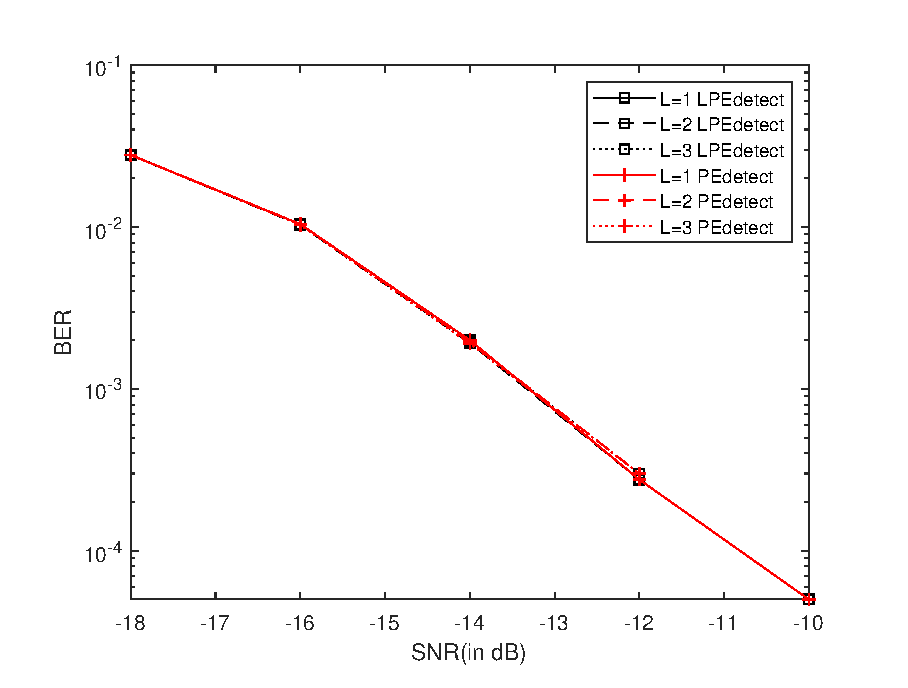
\includegraphics[width=0.45\textwidth]{img/4_5.eps} \caption{4用户单天线LPE接收机与PE接收机比较}
\end{figure}
\begin{figure}[htbp!]
	\centering 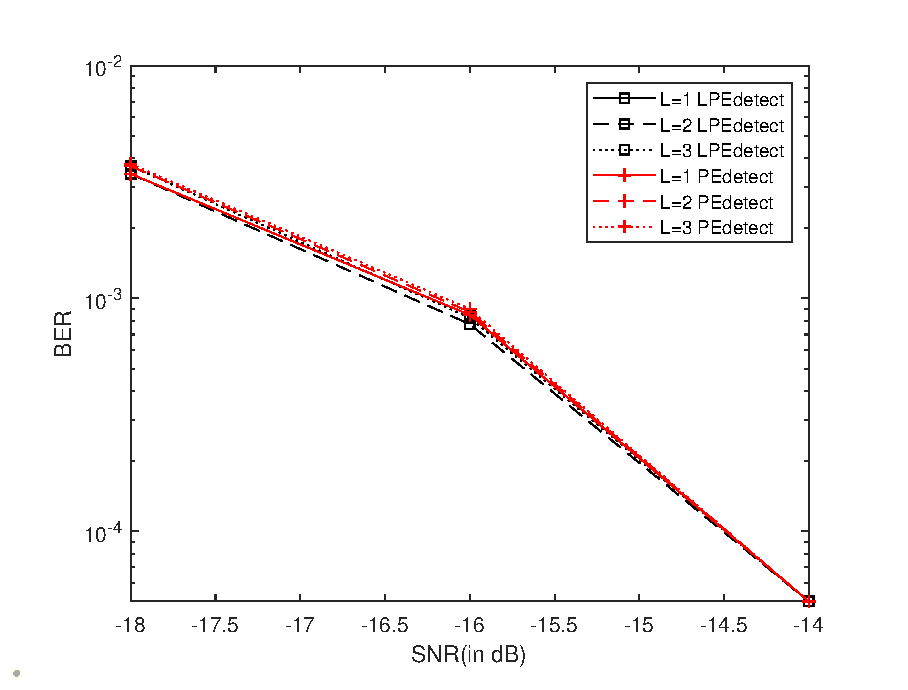
\includegraphics[width=0.55\textwidth]{img/4_6.eps} \caption{4用户2天线单流LPE接收机与PE接收机比较}
\end{figure}

从图4.7,4.9来看,在用户天线数为2,用户数为4时,PE接收机在阶数为4的情况下低复杂度PE接收机能够逼近MMSE接收机的性能,而从图4.10来看在面对用户发送天线数量更多的情况,阶数更高的低复杂度PE接收机会有更好的表现。从图4.8可以看出,可以发现PE接收机与低复杂度PE接收机在阶数比较小的情况下,仍然可以很好的处理不同用户之间带来的干扰。同样的如果考虑的是当用户多天线单流的情况下,低复杂度PE接收机的性能更加接近MMSE接收机。但是低复杂度的PE接收机很难保证多天线多流时的性能。从仿真结果来看,当双天线时,阶数为3的PE的接收机尚能逼近MMSE性能,而低复杂度的PE接收机只能接近阶数为2的PE接收机,而在用户四天线的情况下,阶数为3的PE接收机已经和MMSE的结果产生了差距,需要更高的阶数来应对用户多天线的情况。而低复杂度的PE接收机已经不能很好的接近普通PE接收机,需要更高的阶数去获得更好的性能,由此也可以得到结论,PE接收机与低复杂度PE接收机在处理用户之间的干扰能力性能仍和MMSE持平,但是处理用户天线间干扰尚有优化判断准则的空间,或者需要更高阶数的PE接收机。

\begin{figure}[htbp!]
	\centering 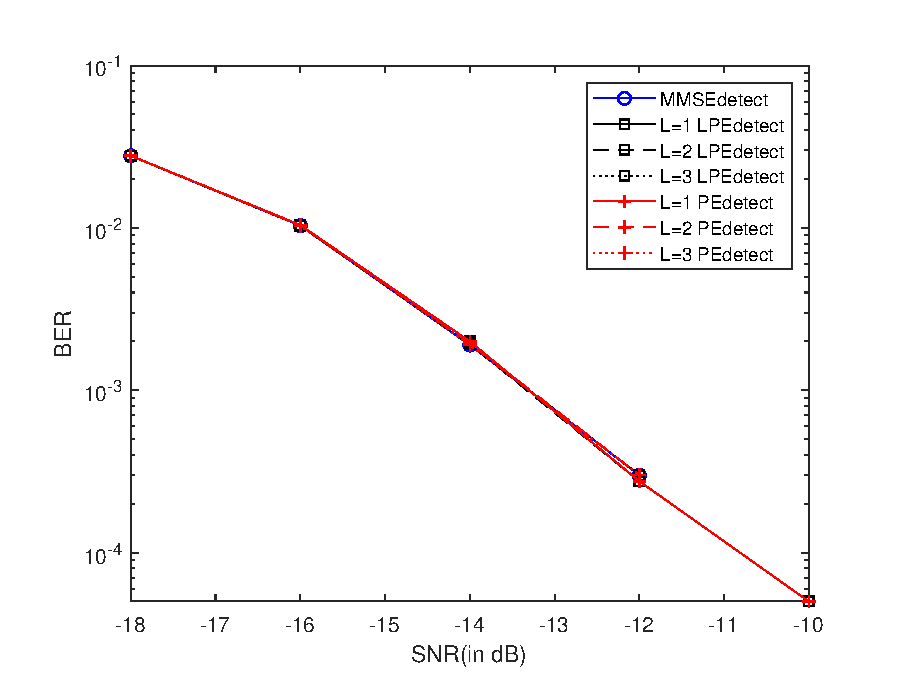
\includegraphics[width=0.55\textwidth]{img/4_8.eps} \caption{4用户单天线LPE接收机与MMSE接收机比较}
\end{figure}
\begin{figure}[htbp!]
	\centering 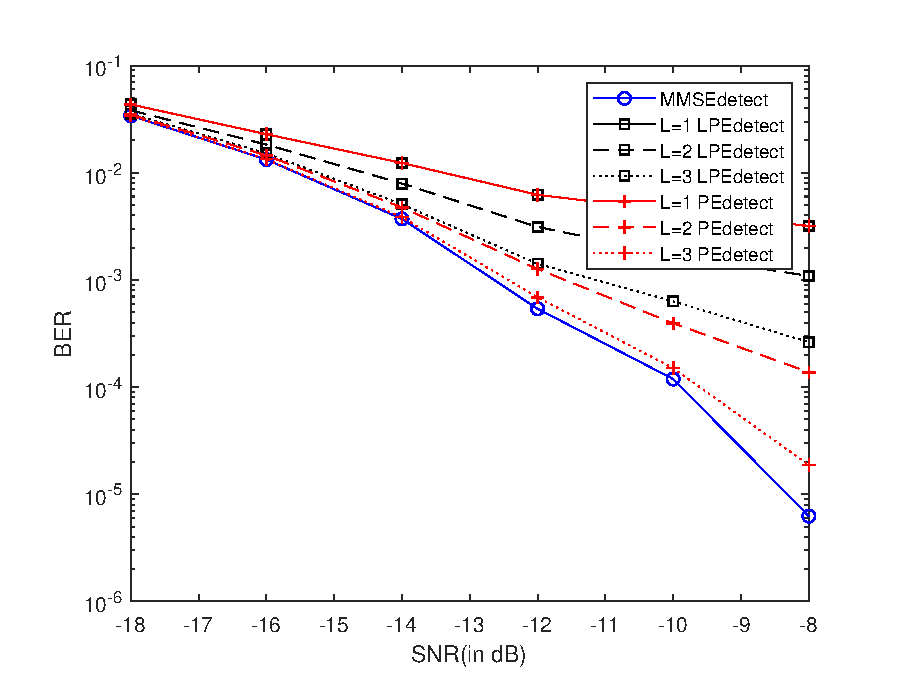
\includegraphics[width=0.55\textwidth]{img/4_12.eps} \caption{16用户单天线LPE接收机与MMSE接收机比较}
\end{figure}
\begin{figure}[htbp!]
	\centering 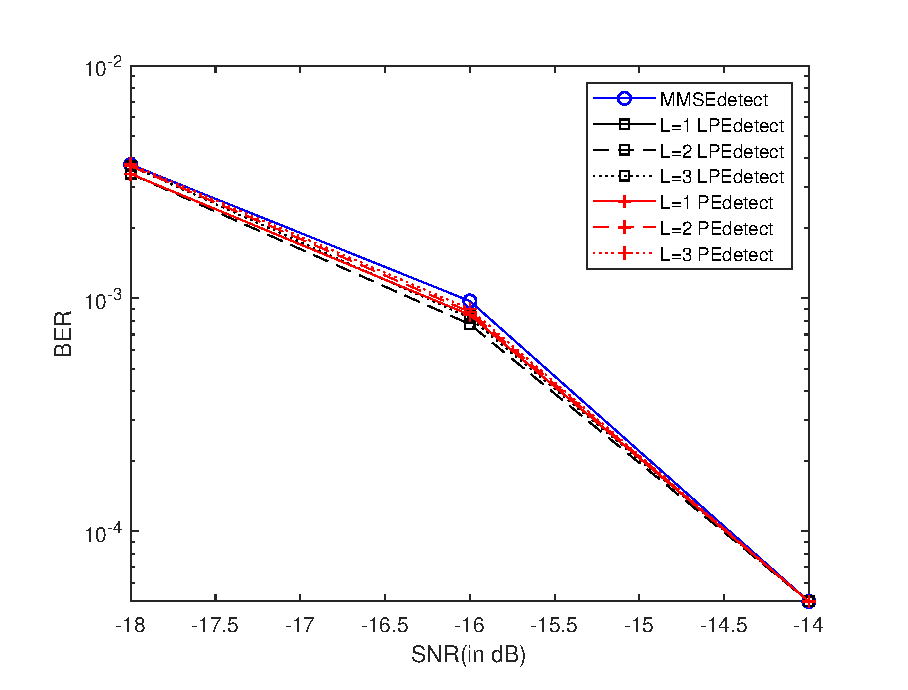
\includegraphics[width=0.55\textwidth]{img/4_9.eps} \caption{4用户2天线单流LPE接收机与MMSE接收机比较}
\end{figure}
\begin{figure}[htbp!]
	\centering 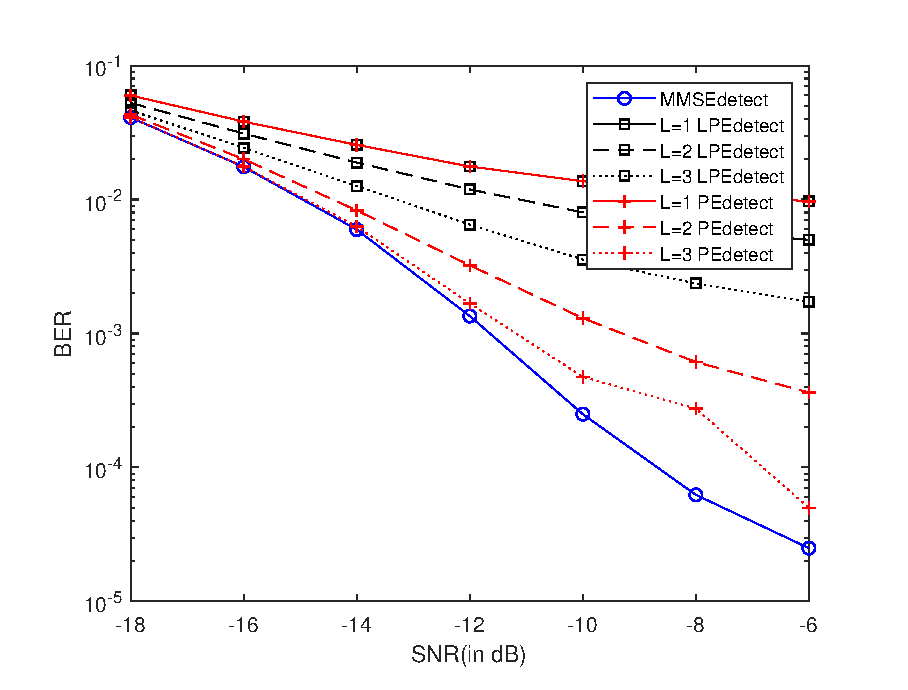
\includegraphics[width=0.55\textwidth]{img/4_10.eps} \caption{4用户2天线多流LPE接收机与MMSE接收机比较}
\end{figure}
\begin{figure}[htbp!]
	\centering 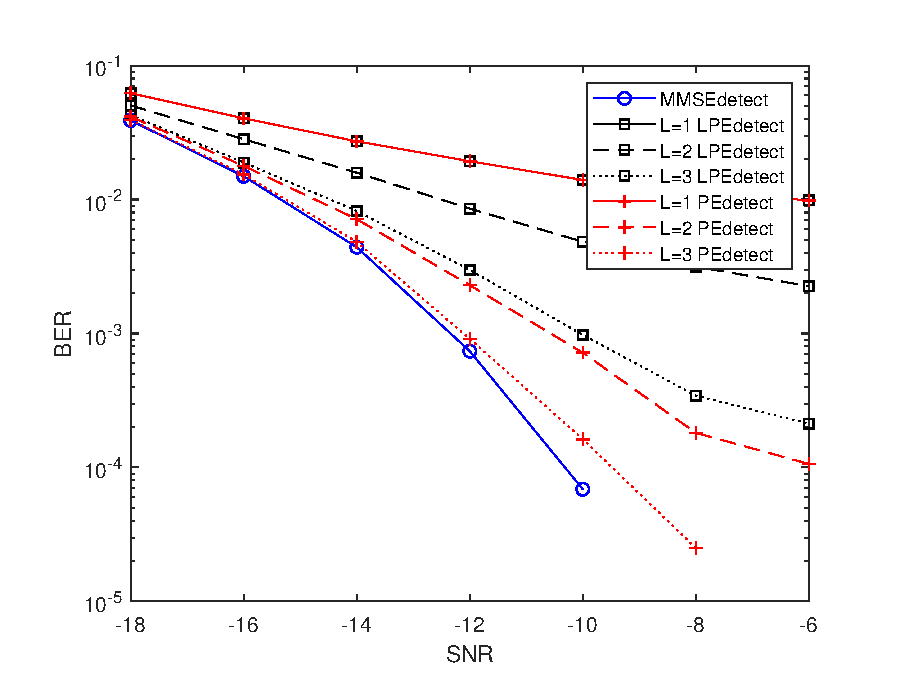
\includegraphics[width=0.55\textwidth]{img/4_11.eps} \caption{4用户4天线多流LPE接收机与MMSE接收机比较}
\end{figure}

\begin{table}[htbp]
	\centering
	\caption{\label{tab:complexity2}PEE复杂度分析表}
	\begin{tabular}{ll}
		\toprule
		方法 & 复杂度 \\
		\bottomrule
		普通MMSE & $O(N_R^3)$ \\
		PE接收机 & $O(N_R^2*L^2)$ \\
		低复杂度PE接收机 & $O(N_R^2)$(与L无关因为只有计算一次确定性等同)\\
		\bottomrule
	\end{tabular}
\end{table}

\section{本章小结}
本章节主要研究了利用Cayley hamilton理论推导的PE接收机,并基于算子自由度理论对其进行了进一步的复杂度降低。首先本文介绍了PE接收机的原理,并且利用第三章推导的系统模型对PE接收机仿真测试,发现PE接收机在降低复杂度的同时能够很好的在阶数较低的情况保持准确度,特别是处理用户间干扰,其结果与MMSE结果。然后本文介绍了算子自由度理论,并根据PE接收机系数可以利用算子自由度理论进行确定性等同替换得到低复杂度的PE接收机,从而进一步降低PE接收机复杂度。根据仿真结果,可以发现低复杂度PE接收机在用户数较少,用户天线数并不多的情况下,是PE接收机的良好替代,并且复杂度得到很大程度的降低。

\chapter{总结与展望}
为了解决通信的数据量猛增以及低损的频谱波段的不足的问题,所以考虑使用大规模多输入多输出传输技术(LS-MIMO Large-Scale Multiple Input Multiple output)。并且第五代通信系统也致力于研究大规模MIMO的技术,所以5G相关的基础技术很多也是和大规模MIMO相关的。
\section{全文总结}
本论文以大规模MIMO技术为背景,主要研究了大规模MIMO系统中信号检测方法,并利用其信道性质和检测数学表达化简得到几种低复杂度的MMSE检测方法。本论文的主要工作总结如下:

首先,在第二章具体阐述了大规模MIMO的系统模型。从物理多径信道模型出发,得到每根接收天线的信道数学表达式,取其集合即为MIMO信道的物理模型,根据MIMO信道采用的多径模型,本文也分析了空间物理信道和统计模型的关系,统计模型是实际上研究与仿真的主要使用的系统模型。然后从MIMO信号,本文过渡到大规模MIMO信道,并且提出了大规模MIMO的波束域信道。然后分析了大规模MIMO波束域信道的三个特征:DFT矩阵解相关,对应波束,特征矩阵稀疏性。本论文使用的3GPP空间信道模型(SCM),设置了具体参数以及得到了波束域仿真信道样本验证了波束域信道的特性。得到了信道模型以及信道性质,为后续章节的研究打下了基础。

其次,在第三章里具体阐述了所使用的系统模型,研究了MMSE接收机和其低复杂度形式。首先根据第二章研究的大规模MIMO的信道模型,提出了大规模MIMO的系统模型,作为本论文所有研究和仿真的基础。
然后本章提出了MMSE检测方法,具体阐述了数学原理和表达式。并利用第二章所介绍的信道仿真SCM模型,进行仿真得到为后续章节作为性能基准的MMSE检测结果。接着,分析MMSE检测数学表达式中复杂度最高的矩阵求逆计算,阐述了利用QR分解的降低复杂度方式。而利用QR分解的Givens变换在稀疏矩阵复杂度降低,以及第二章提到的波束域信道矩阵在经过DFT变换后矩阵稀疏的性质,提出了基于MMSE的低复杂度接收机。利用本章得到的MMSE检测结果与低复杂度的作对比,得出此低复杂度接收机在降低复杂度的同时很好的保持了性能的结论。

最后,在第四章里具体阐述了另一种低复杂度接收机PE接收机及其更低复杂度的确定性等同替换PE接收机。首先,本文利用Cayley Hamilton理论得出了相较MMSE接收机拥有更低复杂度的PE接收机。并利用第三章的系统模型和MMSE检测结果,分析了PE接收机的性能。此时,可以发现PE接收机的系数在利用确定性等同时,在降低复杂度的同时可以保持性能。接着基于算子自由概率理论的具体推导,通过论证得到了确定性等同确实能够很好地代替原来系数。接着,给出了确定性等同的PE接收机表达式,并分析了其复杂度,可以知道低复杂度的PE接收机具有本论文提出的几个低复杂度算法的最好的复杂度。最后利用仿真结果分析了低复杂度PE接收机的性能,以及分析其的不足。

\section{后续工作}
本文对大规模MIMO的检测算法进行研究,检测算法在一定程度降低了计算复杂度,并且分析了很多算法的优势与不足,以及提供了系统模型可以对检测算法进行了分析。进一步的工作包括:
\begin{itemize}
\item[1.]本文并没有在PE接收机上很好的利用波束域信道的特征,并且PE接收机机同样拥有利用波束域信道进行进一步化简的空间,可以在接下来的研究中进一步化简低复杂度的PE接收机。

\item[2.]本文研究的PE接收机的确定等同的算法不是很完善,可以进一步的逼近MMSE估计,后续研究中将进一步完善低复杂度的PE接收机。

\item[3.]本文研究的低复杂度的接收机都有实现在硬件上的潜力,后续可以尝试在硬件上固化这些低复杂度的算法。
\end{itemize}

\end{Main} % 结束正文

% 参考文献
%\bibliographystyle{plain}
\bibliography{seuthesis}

\begin{Acknowledgement}
	在东南学习的四年里,我对信息学科的学习更加深入,对科研产生了浓厚的兴趣,对项目积累了丰富的经验。自己德智体美各方面都得到了长足的进步,也收获很多宝贵的经历。掌握了通信方向的各方面知识,体验了实验研究的各方面工作,这些收获离不开四年里引导我,帮助我的老师同学,离不开背后默默支持我的父母。而现在已经步入毕业阶段,想利用毕设论文的致谢部分对我的父母,老师,同学表达自己最衷心的感谢。
	
	首先我要感谢王闻今老师。最先开始考虑进入实验室的时候,我向班主任表达了我研究生方向想做偏工程一些的诉求,所以推荐了我去找王老师,一开始进入课题组因为不习惯科研研究,并且处于大三事情比较忙碌的时候,科研学习对我来说非常困难。在多次和王老师交流与参与组会时,我慢慢培养起对科研的兴趣和做科研的一些要求和习惯。在课题组学习科研的一年,也给了我很多去接触课题之外许多不同单位实验室的机会,从和他们的沟通交流,我同样收益匪浅。
	
	特别感谢孙晨老师的悉心指导。孙老师主要指导我毕设方向的事情,耐心地指导我,让我了解到课题组一些前沿研究,并一步步从入门带领我到掌握的程度,为我指出了很多论文写作中的错误和不足。孙老师非常细致的指导使得我的毕设研究能够进行非常顺利,为我论文写作提供了巨大的帮助。
	
	衷心感谢尤力老师在我学习生活提供的帮助。作为课题组的老师和班级的班主任,尤力老师给我提供的便利和支持,让我在实验时的科研学习非常的轻松和愉快。组织的各种课题组活动,让我在实验室枯燥的学习生活中还能感受一些轻松愉快的氛围。
	
	特别感谢徐振、吴体昊、石丁、孙榛、李灵瑄、徐益师兄师姐在科研和项目上的帮助,带领我这个科研小白逐渐融入课题组,并且提供了很多科研的经验,让我可以快速上手。感谢师姐杨晓鹤提供的资料,让我更加快速的熟悉项目。感谢同学何思然、杨济源、王一彪、陈婷婷、黄雨菲在实验室的一起科研,让我的科研学习生活非常丰富。感谢我的舍友张皓辰,陈佳伟,严旭阳,在枯燥忙碌的科研学习中总能给我很多愉快,舒适的生活环境和刻骨铭心的记忆。让我在科研之余,能够好好享受大学生活。感谢我的父母,是他们一直在背后默默的支持我,使我能够心无旁骛的学习,科研。是他们的支持、监督和鼓励,让我顺利的完成了学业,并且给我提供了一切可能,是他们的奉献,我才能更好地攀登学业的高峰。
	
	最后感谢东南大学一流的学习、生活和科研环境,使我在东南大学受益匪浅。
	
\end{Acknowledgement}

\newpage
\printindex % 索引

%\begin{thebibliography}{99}



%\bibliography{seuthesis}

 
\end{document}
